\chapter{Results and Discussions}\label{ch:results}
This chapter is organized as follows: Section \ref{sec:result_data} discusses the main data used in this study, including how to access it in the Julia programming language; Section \ref{sec:ch4_desc_stat} presents the results of the descriptive statistics, which include comparisons to the work of \cite{sinai2020oqs}; Section \ref{sec:result_morphological_analysis} explores the results of the morphological analyses, including a deep dive into extant manuscripts containing the three selected morphologies; Section \ref{sec:result_rhythmic_analysis} examines the rhythmic analyses of the Qur'\=an, with particular emphasis on the methodology for analyzing its structural patterns; Section \ref{sec:concentric_structural_optimization} introduces the concept of concentric and chiasmus structures, while Section \ref{sec:result_ga} explains how to find the optimal structural borders of the said structures, and Section \ref{sec:result_thematic_analysis} thematically analyzes these results. Finally, a discussion on the contributions of these computational and mathematical approaches from the lens of Islamic philosophy is provided in Section \ref{sec:result_islamic_philosophy}.
\section{Theoretical Results}
The mathematics of the proposed algorithm used for finding the optimal structural borders of the concentric structures is not provided in this chapter, but is provided in Appendix \ref{appendix:theoretical_results}. This is to avoid cluttering this chapter with heavy mathematics that many Islamic scholars may have difficulty understanding. These results are an original contribution of the paper and are provided in a separate appendix for interested reviewers and readers to understand the inner workings of the algorithm behind the scenes.
\section{Qur'\=an Data}\label{sec:result_data}
The main data used in this study is the digitized Qur'\=an data available through the QuranTree.jl library by \citeA{asaad2021qurantree}. QuranTree.jl has both the Tanzil data\footnote{\url{https://tanzil.net/}} and the Qur'anic Arabic Corpus\footnote{\url{https://corpus.quran.com/}}, where the latter contains the morphological data of the Qur'\=an. These digital data will help in doing programmatic analyses of the Qur'\=an using the Julia programming language. To see how to access this in QuranTree.jl in Julia, Listing \ref{lst:result_crps_tbl} shows the code for accessing the morphological data of the first \arb[trans]{'ayaT} \arb{'ayaT} of \arb[trans]{sUraTu 'l-fAti.haT} \arb{sUraTu 'l-fAti.haT}. Note that the setup on how to install the said QuranTree.jl and other libraries and the Julia programming language is given in Appendix \ref{appendix:installation_libraries}.

Referring to Listing \ref{lst:result_crps_tbl}, the first line of the code, which has the code \texttt{using QuranTree}, loads the QuranTree library. The second line, which has the code \texttt{crps, tnzl = load(QuranData())}, loads both the morphological data and the Tanzil data of the Qur'\=an. The third line of the code converts these data into a tabular form. Finally, the fourth line of the code queries the first \arb[trans]{sUraT} \arb{sUraT} and the first \arb[trans]{'ayaT} \arb{'ayaT} of the morphological data of the Qur'\=an, the results of which are shown in the succeeding lines with the heading indicating \texttt{Chapter 1} and \texttt{Verse 1}. The number 1 for Chapter 1 and Verse 1 are indicated by \texttt{[1]} and \texttt{[1]}, respectively, in the code \verb|crps_tbl[1][1]| in Listing \ref{lst:result_crps_tbl}.

\begin{listing2}[!t]
    \centering
    \includegraphics[width=\textwidth]{img/crps_tbl.png}
    \caption{\arb[trans]{sUraTu 'l-fAti.haT} \arb{sUraTu 'l-fAti.haT} morphological data}
    \label{lst:result_crps_tbl}
\end{listing2}

The output of the code in Listing \ref{lst:result_crps_tbl} as indicated by the lines starting with \texttt{\#} shows the morphological data of the \textit{basmallah} \arb[fullvoc]{bismi 'l-l_ahi 'l-ra.hm_ani 'l-ra.hImi}. In this data, there are five columns after the Row column. The \texttt{word} column indicates the word of the queried data, in this case the first \arb[trans]{'ayaT} \arb{'ayaT} of the first \arb[trans]{sUraT} \arb{sUraT}. According to this column, there are four words in the \textit{basmallah}. The second column, \texttt{part}, indicates the parts of the word. In this case, the first word has two parts. These two parts are indicated by their \texttt{form} in the third column, which are \texttt{bi}, a Roman encoding based on Buckwalter \cite{buckwalter2002} mapping which is decoded in Arabic as \arb{bi}, and the second part of the first word has the form in Roman encoding through Buckwalter as \texttt{somi} or decoded in Arabic as \arb[trans]{smi} \arb[fullvoc]{smi}. The fourth column indicates the part-of-speech of the parts of the words. For the first word, \arb[trans]{bismi} \arb[fullvoc]{bismi}, its two parts are composed of a Preposition \arb[trans]{bi} \arb{bi} and a Noun \arb[trans]{smi} \arb[fullvoc]{smi}, both of which are further described in the \texttt{features} column, which contains the morphological features of the part of the given word. In this last column, it further tells the reader that the Preposition \arb[trans]{bi} \arb{bi} is a prefix. In addition, the second part \arb[trans]{smi} \arb[fullvoc]{smi} is the stem of the word \arb[fullvoc]{bismi}, with the lemma indicated by \texttt{\{som} which is decoded as \arb[trans]{"ism} \arb{"ism}, and a root of \arb[trans]{smw} \arb{smw}. There are still other features detailed in the morphological column for the second word \arb[trans]{smi} \arb[fullvoc]{smi}, and these can be described further using QuranTree.jl's \texttt{@desc} macro. The result of which is given in Listing \ref{lst:result_at_desc_basmallah}, which also shows the other features such as the gender of the noun, in this case it is Masculine and is in Genitive case.

\begin{listing2}[!t]
    \centering
    \includegraphics[width=\textwidth]{img/at_desc_basmallah.png}
    \caption{Morphological features of the second part of the word \arb[trans]{bismi} \arb[fullvoc]{bismi}}
    \label{lst:result_at_desc_basmallah}
\end{listing2}

The Quranic Arabic Corpus data which contains the morphological features discussed above, has the Qur'\=an texts represented as Buckwalter encoding, which is a character by character mapping of the Arabic orthographies of the Qur'\=an into Roman letters. This encoding, if decoded to Arabic, matches exactly the Qur'\=an \arb[trans]{mu.s.haf} \arb{mu.s.haf}. In fact, the Tanzil data which is also available in QuranTree.jl \cite{asaad2021qurantree}, exactly matches this data. The difference between the two is that the Tanzil data only contains the Arabic texts of the Qur'\=an broken down up to the \arb[trans]{'ayaT} \arb{'ayaT} level only. Listing \ref{lst:result_tnzl_tbl} shows the Tanzil data queried through the QuranTree.jl \cite{asaad2021qurantree} for \arb[trans]{sUraTu 'l-fAti.haT} \arb{sUraTu 'l-fAti.haT}. The only difference between the two data sources in terms of presentation of the \arb[trans]{sUraT} \arb{sUraT} is that the Quranic Arabic Corpus (in Listing \ref{lst:result_crps_tbl}) skips the \textit{basmallah} for all \arb[trans]{sUwar} \arb{sUwar} except for the first, \arb[trans]{sUraTu 'l-fAti.haT} \arb{sUraTu 'l-fAti.haT}, while the Tanzil data has it in every \arb[trans]{sUwar} \arb{sUwar}.

\begin{listing2}[!t]
    \centering
    \includegraphics[width=\textwidth]{img/tnzl_tbl.png}
    \caption{\arb[trans]{sUraTu 'l-fAti.haT} \arb{sUraTu 'l-fAti.haT} Tanzil data}
    \label{lst:result_tnzl_tbl}
\end{listing2}

The rich data available in QuranTree.jl \cite{asaad2021qurantree} opens up many possibilities for researchers to do programmatic analyses of the Qur'\=an, especially for the use of Statistical modeling to understand its structure and patterns.
\section{Descriptive Statistics}\label{sec:ch4_desc_stat}
The first statistical analysis is to describe the distribution of the data through Descriptive Statistics. This statistical method is mainly used to summarize the data by looking at the central tendency, dispersion, and shape of the distribution. The central tendency is a measure of the center of the data, which can be represented by the mean, median, and mode. The dispersion is a measure of how spread out the data is, which can be represented by the range, variance, and standard deviation.

The data in this case are the orthographies, parts of words, words, \arb[trans]{'AyAt} \arb{'AyAt}, and \arb[trans]{sUraT} \arb{sUraT} of the Qur'\=an. The Qur'\=an is a collection of 114 \arb[trans]{suwar} \arb{suwar} and 6,348 \arb[trans]{'AyAt} \arb{'AyAt}. Each \arb[trans]{sUraT} \arb{sUraT} is made up of a number of \arb[trans]{'AyAt} \arb{'AyAt}, and each \arb[trans]{'AyAt} \arb{'AyAt} is made up of a number of words, which in turn are made of parts, and finally, parts are made up of Arabic letters. These data, as discussed in the previous section, are available through the Quranic Arabic Corpus and the Tanzil data in the QuranTree.jl library.

Moving on, the Qur'\=an has a unique organizational structure that is totally different from other scriptures. This uniqueness has attracted both Muslims and non-Muslims to dive deeper to understand the design of its presentation. The typical approach even to this day is to do this manually, going through each \arb[trans]{'AyAt} \arb{'AyAt} and \arb[trans]{sUraT} \arb{sUraT} of the Qur'\=an one at a time to find patterns that will at least convey why it is arranged as it is. As expected, this manual process is very tedious and time-consuming, and may missed some data points in the process if not done carefully. However, with the advent of computations, slowly and especially recently, some automation can now be done to do repeatetive tasks of finding patterns. Among the researchers to understanding the structure of the Qur'\=an is by studying the statistics of the counts of words, \arb[trans]{'AyAt} \arb{'AyAt}, and \arb[trans]{suwar} \arb{suwar}.

\begin{figure}[!t]
    \centering
    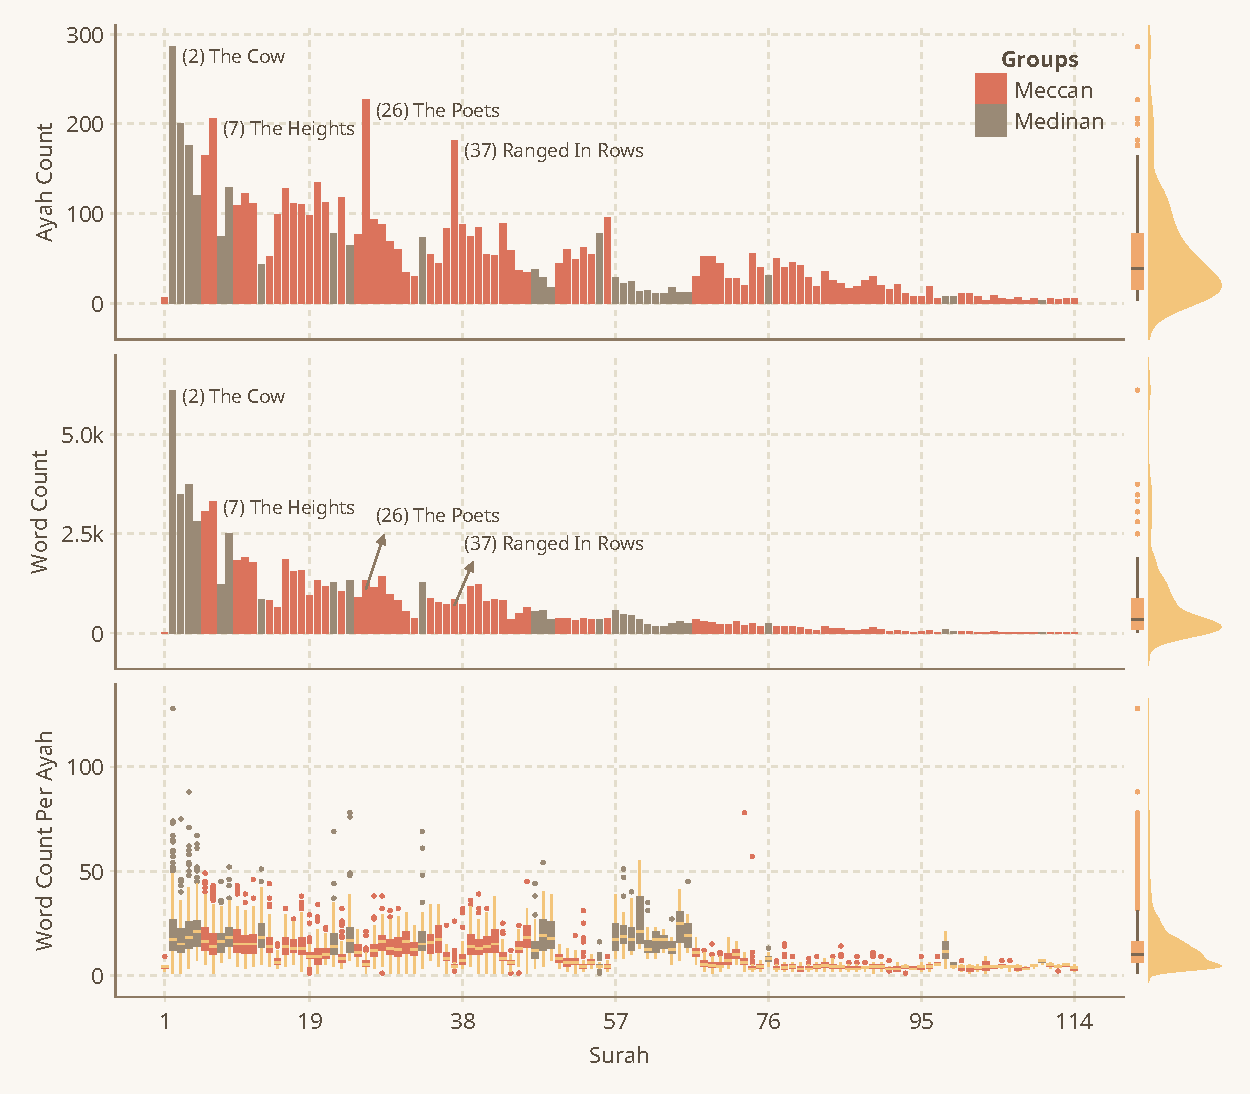
\includegraphics[width=\textwidth]{img/plot1.pdf}
    \caption{Distribution of Meccan and Medinan \arb[trans]{sUwar} \arb{suwar}}
    \label{fig:result_ayah_word_count}
\end{figure}

Figure \ref{fig:result_ayah_word_count} shows the bar chart of the \arb[trans]{'AyAt} \arb{'AyAt} counts and word counts, as well as the distribution of the word counts and character counts per \arb[trans]{'AyAt} \arb{'AyAt}. In this figure, the geographical locations (Meccan or Medinan) of the \arb[trans]{sUraT} \arb{sUraT} based on the \arb[trans]{'asbAb 'alnuzUl} \arb{'asbAb 'alnuzUl} or the 'occasions/circumstances of revelation' are also indicated.

The first obvious pattern in Figure \ref{fig:result_ayah_word_count}, which is known to Muslims, is the monotonically decreasing number of \arb[trans]{'AyAt} \arb{'AyAt} after the first \arb[trans]{sUraT} \arb{sUraT}. This is true for both the bar charts of the \arb[trans]{'AyAt} \arb{'AyAt} count and the word count. There are, however, interesting pattern in the first two plots of the said figure, and that is two \arb[trans]{suwar} \arb{suwar} having significant number of \arb[trans]{'AyAt} \arb{'AyAt} but each having small number of words. These two \arb[trans]{suwar} \arb{suwar} are the 26th \arb[trans]{sUraT} \arb{sUraT} (\arb[trans]{sUraTu 'l-^su`arA'} \arb{sUraTu 'l-^su`arA'} or "the Poet") and 37th \arb[trans]{sUraT} \arb{sUraT} (\arb[trans]{sUraTu 'l-.sAffAt} \arb{sUraTu 'l-.sAffAt} or "the Ranged in Rows"), respectively. This can be confirmed even in the Medina Mushaf, where the first page for \arb[trans]{sUraTu 'l-^su`arA'} \arb{sUraTu 'l-^su`arA'} already contains 19 \arb[trans]{'AyAt} \arb{'AyAt}, and the \arb[trans]{sUraTu 'l-.sAffAt} \arb{sUraTu 'l-.sAffAt} contains 24 \arb[trans]{'AyAt} \arb{'AyAt} in its first page. This indicates that the said \arb[trans]{suwar} \arb{suwar} contain a small number of words per \arb[trans]{'AyAt} \arb{'AyAt}, as shown in Figure \ref{fig:result_ayah_word_count}.

Moving on, the distribution of words per \arb[trans]{'AyAt} \arb{'AyAt} and characters per \arb[trans]{'AyAt} \arb{'AyAt} are shown in the third and fourth rows or plots of Figure \ref{fig:result_ayah_word_count}. It is indeed expected that these distributions are more or less identical, since more words typically mean more characters. The distribution of characters per \arb[trans]{'AyAt} \arb{'AyAt} is shown to make it comparable to the work of \citeA{sinai2020oqs}, which will be discussed in Section \ref{sec:comparison_sinai}.

\begin{figure}[!t]
    \centering
    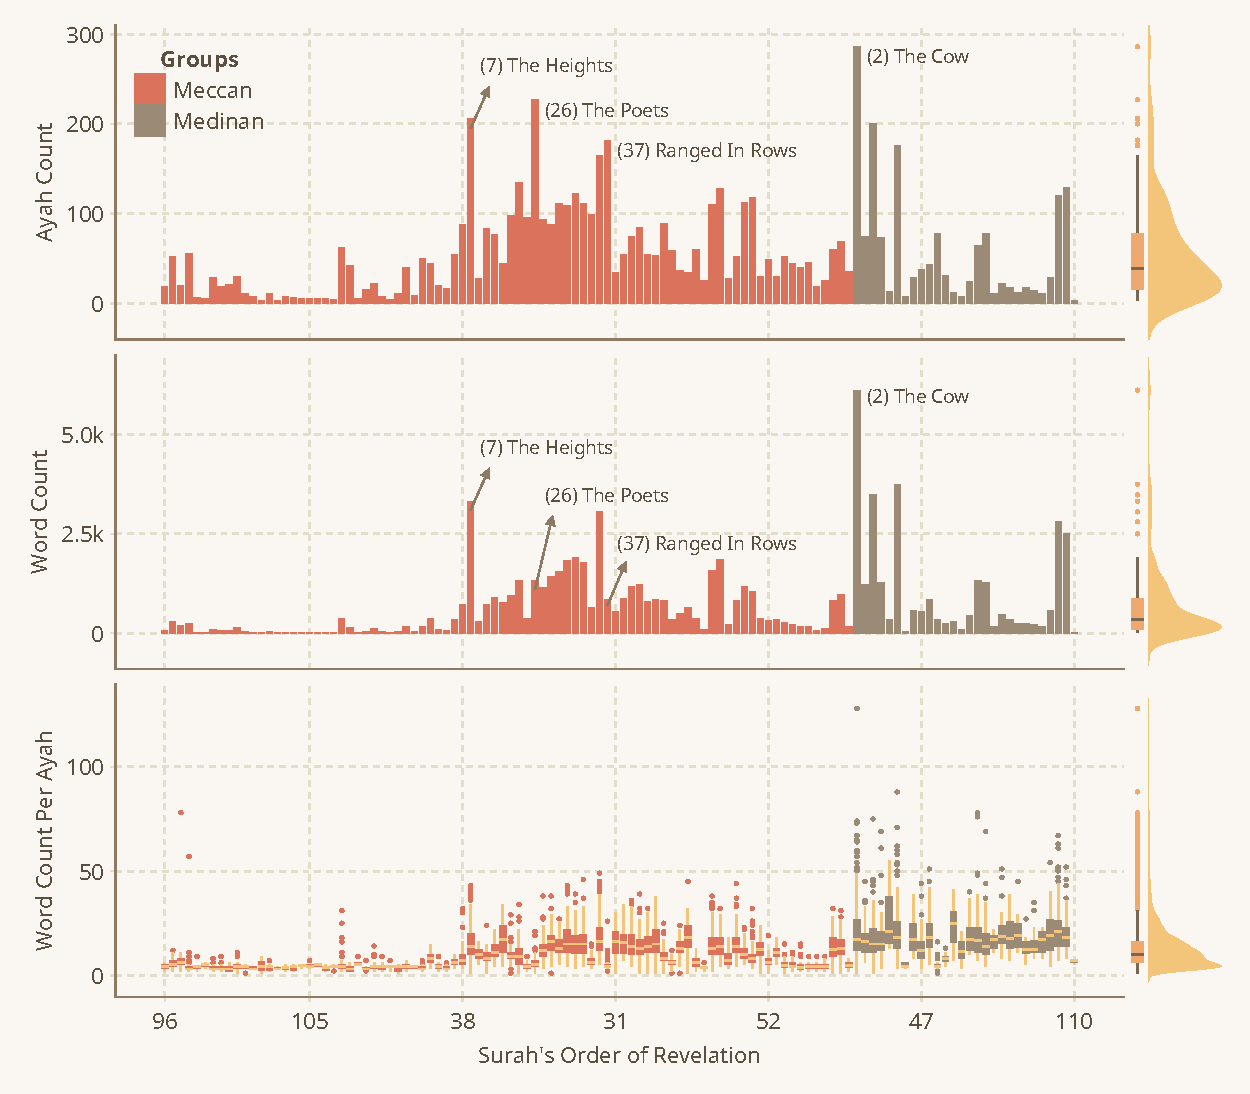
\includegraphics[width=\textwidth]{img/plot2.pdf}
    \caption{Statistics of the words and \arb[trans]{'AyAt} \arb{'AyAt} (verses) of the Qur'\=an according to revelation order}
    \label{fig:result_ayah_word_count_rev_order}
\end{figure}

To help interpret the plots for the distributions of word count per \arb[trans]{'AyAt} \arb{'AyAt} and character count per \arb[trans]{'AyAt} \arb{'AyAt} in Figure \ref{fig:result_ayah_word_count}, the $x$-axis represents the 114 \arb[trans]{suwar} \arb{suwar} of the Qur'\=an, while the $y$-axis represents either the count of words (third row plot) per \arb[trans]{'AyAt} \arb{'AyAt} or the count of characters (fourth row plot) per \arb[trans]{'AyAt} \arb{'AyAt} in Figure \ref{fig:result_ayah_word_count}. Thus, each boxplot shown in these plots describes the distribution of the count of either words (third row plot) or characters (fourth row plot) per \arb[trans]{'AyAt} \arb{'AyAt}. From these distributions, interesting groups of distributions are observed around the 57th to 66th \arb[trans]{sUraT} \arb{sUraT}. While the color of these distributions helped in distinguishing it as \arb[trans]{madaniyyaT} \arb{madaniyyaT} (or Medinan) based in \arb[trans]{'asbAb 'alnuzUl} \arb{'asbAb 'alnuzUl}, the mean of these \arb[trans]{madaniyyaT} \arb{madaniyyaT} \arb[trans]{suwar} \arb{suwar} is observed to be higher than that of the surrounding \arb[trans]{sUraT} \arb{sUraT}, as seen in the figure. In fact, these \arb[trans]{suwar} \arb{suwar} have a lower number of \arb[trans]{'AyAt} \arb{'AyAt} compared to the surrounding \arb[trans]{makkiyyaT} \arb{makkiyyaT} \arb[trans]{suwar} \arb{suwar} (\textit{see} first row plot and second row plot of Figure \ref{fig:result_ayah_word_count}), which has opposing patterns, and that is, those \arb[trans]{madaniyyaT} \arb{madaniyyaT} \arb[trans]{suwar} \arb{suwar} has variable number of words or characters per \arb[trans]{'ayaT} \arb{'ayaT}, while those \arb[trans]{makkiyyaT} \arb{makkiyyaT} \arb[trans]{suwar} \arb{suwar} tend to have lower variable variability in the number of words or characters. Indeed, even the 98th \arb[trans]{sUraT} \arb{sUraT}, which is a \arb[trans]{madaniyyaT} \arb{madaniyyaT}, sticks out significantly due to its high variability compared to its surrounding \arb[trans]{makkiyyaT} \arb{makkiyyaT} \arb[trans]{suwar} \arb{suwar} which have more or less similar number of words and \arb[trans]{'AyAt} \arb{'AyAt}. There are some exception though, for example the 55th and 99th \arb[trans]{suwar} \arb{suwar}, which both have small variability, but the rest tend to have a higher variability in the number of words or characters per \arb[trans]{'ayaT} \arb{'ayaT}, even the 110th \arb[trans]{sUraT} \arb{sUraT}, which at glance seem to be part of the excemption, but relative to its neighbour it still has a higher variability despite having only three \arb[trans]{'AyAt} \arb{'AyAt}. 

In addition, when re-arranged according to its order of revelation as in Figure \ref{fig:result_ayah_word_count_rev_order}, the \arb[trans]{madaniyyaT} \arb{madaniyyaT} grouped towards the end shows the same pattern of higher variability. Indeed, when grouping all of these data points into its \arb[trans]{'asbAb 'alnuzUl} \arb{'asbAb 'alnuzUl}, the corresponding distributions are given in Figure \ref{fig:result_meccan_medinan_dist}. In the said figure, it clearly shows that those \arb[trans]{madaniyyaT} \arb{madaniyyaT} \arb[trans]{suwar} \arb{suwar} have higher central tendency as indicated by its median, and also has higher variability as indicated by its wide range. This findings is supported by Table \ref{tbl:desc_stats}, where the average word counts per \arb[trans]{'AyAt} \arb{'AyAt} is higher (median of 18.10) for \arb[trans]{madaniyyaT} \arb{madaniyyaT} compared to that of \arb[trans]{makkiyyaT} \arb{makkiyyaT} (median of 5.81). In addition to this, the standard deviation of the average word counts per \arb[trans]{'AyAt} \arb{'AyAt} is also higher (std. of 5.66) for \arb[trans]{madaniyyaT} \arb{madaniyyaT} compared to that of \arb[trans]{makkiyyaT} \arb{makkiyyaT} (std. of 4.90).

\begin{table}[!t]
    \caption{Descriptive statistics of the \arb[trans]{'AyAt} \arb{'AyAt} for \arb[trans]{makkiyyaT} \arb{makkiyyaT} and \arb[trans]{madaniyyaT} \arb{madaniyyaT}}
    \label{tbl:desc_stats}
    \begin{tabularx}{\textwidth}[!h]{lcccXccc}
        \toprule
        &\multicolumn{3}{c}{\textbf{\arb[trans]{makkiyyaT} \arb{makkiyyaT}}}&&\multicolumn{3}{c}{\textbf{\arb[trans]{madaniyyaT} \arb{madaniyyaT}}}\\[0.15cm]\cline{2-4}\cline{6-8}\\[-0.3cm]
        \textbf{Variables}&\textbf{Mean}&\textbf{Median}&\textbf{Std.}&&\textbf{Mean}&\textbf{Median}&\textbf{Std.}\\[0.1cm]
        \midrule
        Ayah Counts&53.63&43&47.77&&57.96&29&68.21\\
        Word Counts&10.28&8&7.36&&18.48&16&11.71\\
        Ave. Words per Ayah&8.10&5.81&4.90&&16.93&18.10&5.66\\
        Ave. Chars. per Ayah&64.33&45.60&38.46&&139.48&150.14&46.39\\
        \bottomrule
    \end{tabularx}
\end{table}

\begin{figure}[!t]
    \centering
    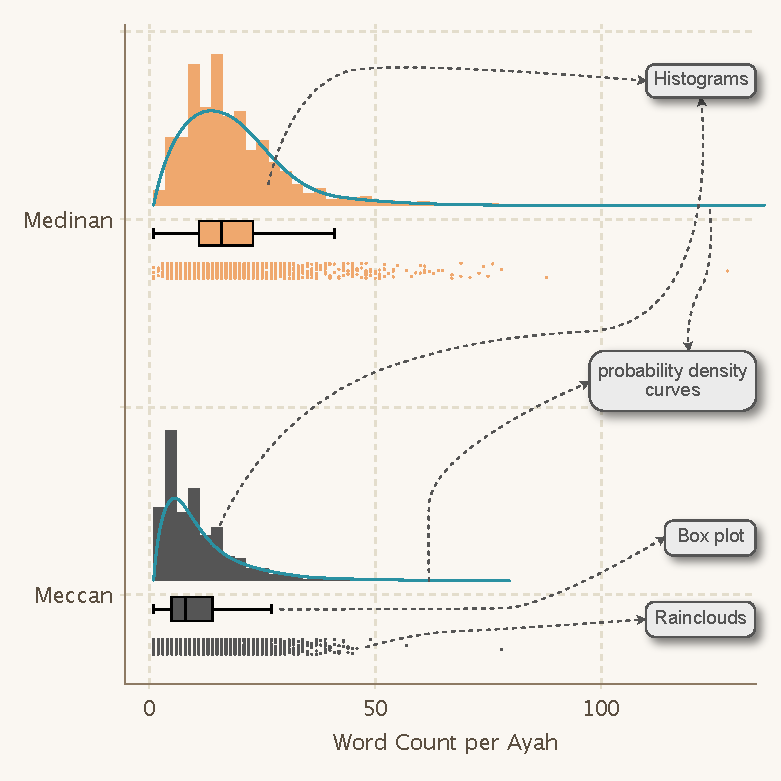
\includegraphics[width=\textwidth]{img/plot3.pdf}
    \caption{Distribution of Meccan and Medinan \arb[trans]{sUwar} \arb{sUwar}}
    \label{fig:result_meccan_medinan_dist}
\end{figure}

Furthermore and diving deep into the variability of these two types of \arb[trans]{'asbAb 'alnuzUl} \arb{'asbAb 'alnuzUl}, Figure \ref{fig:result_scatter_variabilities} shows different perspectives on the characteristics of \arb[trans]{makkiyyaT} \arb{makkiyyaT} and \arb[trans]{madaniyyaT} \arb{madaniyyaT}. In the said figure, the variable \arb[trans]{suwar} \arb{suwar} in terms words per \arb[trans]{'ayaT} \arb{'ayaT} versus the \arb[trans]{'AyAt} \arb{'AyAt} counts and the word counts are mostly \arb[trans]{madaniyyaT} \arb{madaniyyaT}. This is clearly seen in blue points almost consistently at the top of red points for every \arb[trans]{'AyAt} \arb{'AyAt} counts and the word counts in the said figure. This is true even for character variability, or even in the three-dimensional perspective with the added \arb[trans]{sUraT} \arb{sUraT}. Overall, the statistics and the different statistical visualizations used clearly show distinction of the two \arb[trans]{'asbAb 'alnuzUl} \arb{'asbAb 'alnuzUl}, and that is the two have differing \arb[trans]{'ayaT} \arb{'ayaT} length variability. The next section will compare this result to other theories from orientalist, in this case \cite{sinai2020oqs}.

\begin{figure}[!t]
    \centering
    \includegraphics[width=\textwidth]{img/plot6.pdf}
    \caption{Scatter Plots of Word and Character Variabilities Against Surah and Word Counts}
    \label{fig:result_scatter_variabilities}
\end{figure}

\subsection{Comparison to Sinai's Inner-Chronology}\label{sec:comparison_sinai}
\citeA{sinai2020oqs} investigated the same statistical distributions as in the previous section, though with slight statistical measurement used, which will be discussed later. His work is based from a different premise. Instead of relying on the \arb[trans]{'asbAb 'alnuzUl} \arb{'asbAb 'alnuzUl} as believed by Muslims, he decided to ignore it and instead rely on the Qur'\=an's texts itself. The following is the reasoning,

\begin{quotation}
    \noindent . . . I shall try to delineate the main
    contours of a chronological approach to the Qur'\=an by engaging with a recent critique of
    it \cite{LeproblmedelachronologieduCoran1}. For Reynolds, the continuity between Weil and Nöldeke's work and
    the earlier Islamic tradition is indicative of the fact that all Western attempts at a relative
    dating of Qur'\=anic texts are irredeemably reliant on Islamic reports about the biography
    (sīra) of Muḥammad \txarb{\fontspec{Scheherazade New} ﵇}: scholars who work with a chronological model perpetuate the
    established Islamic practice of making sense of the Qur'\=an by linking it up with apocryph­al 
    extra-Qur'\=anic traditions. Although Reynolds acknowledges that both Nöldeke
    and Régis Blachère profess to build their chronological reconstructions on observations
    internal to the Qur'\=anic text \cite<p. 486, 490-1>{LeproblmedelachronologieduCoran1}, he is unconvinced that they
    succeed in implementing this principle. For example, Reynolds points out that
    Blachère's invocation of the terminological distinction between `the Israelites' (banū
    Isrā'īl), considered to be a typically Meccan expression, and `the Jews' (al-yahūd), considered to be Medinan, 
    is anchored in the assumption that the Qur'\=anic texts revealed in
    Medina would naturally have been less interested in 'the ancient Hebrews and their
    descendants' than in 'the small Jewish communities of that town' (Reynolds 2011: 491,
    quoting Blachère). Blachère's neat assignment of two easily identifiable terms to the
    Qur'\=an's two main stages of composition thus turns out to be predicated on extra-Qur'\=anic information about the Medinan suras' confessional environment: the terminological observation that certain suras prefer the expression 'Israelites' to 'Jews' becomes
    chronologically relevant only by covertly hooking it up with the historical power generator
    of the sīra. 
\end{quotation}

\noindent\citeA{sinai2020oqs} further states the following:

\begin{quotation}
    Chronological readings of the Qur'\=an, as portrayed by Reynolds, invariably
    seem to proceed in this fashion: Qur'\=anic terms, themes, and stylistic peculiarities are
    more or less uncritically assigned to the stages of Muḥammad's \txarb{\fontspec{Scheherazade New} ﵇} career as known from
    the sīra tradition. Whether a consistent bracketing of the sīra would leave behind any
    foundation on which to base meaningful chronological statements must thus appear
    doubtful.
\end{quotation}

The argument made by Reynold as how it is described above by \cite{sinai2020oqs} are not meant to disprove the credibility of the \arb[trans]{'asbAb 'alnuzUl} \arb{'asbAb 'alnuzUl}, what Reynold is saying is that the the geographical locations or environment or stages of Prophet Muhammad's \txarb{\fontspec{Scheherazade New} ﵇} career may not be of critical dependence for the terms, themes, and stylistic pecularities of the Qur'\=an. So that, instead of studying the styles of the Qur'\=an based on these categorization, it maybe better to study the structure and styles directly from the texts itself. This led \cite{sinai2020oqs} to developing what he called the inner-chronology of the Qur'\=an. In particular, Sinai used the transliterated text data from Prof. Hans Zirker. The said data is not exactly the same as the one used in here, nor is it publicly verified as the one (Quranic Arabic Corpus and the Tanzil data) used in this study. Nonetheless, if indeed the said transliteration is exactly the same as the one used here once decoded to its Arabic form, the result should more or less be the same. However, while the preprocessing done by \citeA{sinai2020oqs} was not done in the analyses of the previous section, the result of the distributions should not deviate much. In the said study of \citeA{sinai2020oqs}, the findings suggest that there is inner-chronology of the Qur'\=an. This was concluded by the said author by looking at the mean verse length, which is more or less similar to the median verse length indicator used in boxplots of the third and fourth plots of Figures \ref{fig:result_ayah_word_count} and \ref{fig:result_ayah_word_count_rev_order}. Indeed, median is a better metric than mean in this case due to outlier counts seen in the boxplots in Figures \ref{fig:result_ayah_word_count} and \ref{fig:result_ayah_word_count_rev_order}.

The inner-chronology of the Qur'\=an simply states that as the mean of the word increases, the variability of the characters (even words as will be shown later) per \arb[trans]{'AyAt} \arb{'AyAt} also increases. The way he did this was through the use of standard deviation and coefficient of variation as the measure of variabilities, and plotted this using bar graph with double bar, where $x$-axis as the mean verse length and $y$-axis as the mean (first bar) and also serves as the axis for standard deviation (second bar). Further, he also used the 95\% confidnece interval range for describing this variability as the $y$-axis. He argued that a \arb[trans]{sUraT}'s \arb{sUraT} mean \arb[trans]{'ayaT} \arb{'ayaT} length is a \textit{chronologically significant stylistic marker}, that is, two \arb[trans]{suwar} \arb{suwar} whose confidence interval do not overlap would therefore normally---\textit{ceteris paribus}---be considered not to be contemporaneous. 

Now, let's investigate his findings. While the bar plot used is indeed one way to show this inner-chronology of the Qur'\=an, but the appropriate visualization for studying the relationship of the mean \arb[trans]{'ayaT} \arb{'ayaT} length versus the \arb[trans]{'AyAt} \arb{'AyAt} variability is through a scatter plot. Figure \ref{fig:result_sinai_chronology} shows the said visualization. Here, there are four plots. The first row corresponds to the mean of the characters per \arb[trans]{'ayaT} \arb{'ayaT}, while the second row corresponds to the mean of the words per \arb[trans]{'ayaT} \arb{'ayaT}. Further, while the work of Sinai did not indicate the \arb[trans]{'asbAb 'alnuzUl} \arb{'asbAb 'alnuzUl}, here we indicate it for comparison. From the said figure, there is indeed strong correlation between the mean \arb[trans]{'ayaT} \arb{'ayaT} length and its variability. This is seen when fitting a regression line as shown in the second column of the said figure.

\begin{figure}[!t]
    \centering
    \includegraphics[width=\textwidth]{img/plot7.pdf}
    \caption{Mean Ayah Length vs. Its Ayah Variability With Outlier Comparison}
    \label{fig:result_sinai_chronology}
\end{figure}

Moreover, one of Sinai's findings are \arb[trans]{suwar} \arb{suwar} with high variability in relation to their chronological mean \arb[trans]{'ayaT} \arb{'ayaT} length marker. These \arb[trans]{suwar} \arb{suwar} were the following: Q83, Q103, Q53, Q73, and Q74. In particular, according to Sinai the five \arb[trans]{suwar} \arb{suwar} have coefficient of variations above 76 percent. The passages from these \arb[trans]{suwar} \arb{suwar} according to Sinai were the following: Q52:21, Q53:23, Q53:26-32, Q69:7, Q73:20, Q74:31, Q74:56, Q78:37-40, Q81:29, Q84:25, Q85:7-11, Q87:7, Q89:15-16, Q89:23-24, Q89:27-30, Q90:17-20, Q95:6, Q97:4, and Q103:3. Further, he claims the following regarding the listed \arb[trans]{'AyAt} \arb{'AyAt}:
\begin{quotation}
    A close examination of these verses makes it plausible to consider them as later insertions, many of which serve to comment on or qualify other parts of the sura in which they occur.
\end{quotation}

Such claim though requires strong evidence, and while Sinai cited some of his work to justify this, but his reasoning above suggests that the investigation he did were mainly textual analysis, and not investigation of extant manuscripts containing those claimed 'insertions.' It is unfortunately problematic since to say \textit{later insertion} should be based at least on extant manuscript and not on none conformity of one \arb[trans]{'ayaT} \arb{'ayaT} length relative to a particular assumed chronological marker, in this case the mean \arb[trans]{'AyAt} \arb{'AyAt} length. Sinai is a proponent of \textit{historical-critical perspective} of studying the Qur'\=an, but this approach of not looking at the extant manuscript (which contains the history) and instead depending on statistics as basis for plausible insertions is hard to agree on.

As shown in Figure \ref{fig:result_sinai_chronology}, these outliers found by \cite{sinai2020oqs} are shown in the first column of the said figure. If one uses a statistical outlier detection, like the Least Trimmed Square (LTS), one would find that there are many other possible \arb[trans]{suwar} \arb{suwar} that can be considered as outliers. However, using these as basis for textual analysis and concluding it as plausible insertion is so far-off unfortunately. The main reason could be his use of 95\% confidence interval as basis as opposed to using scatter plot approach as provided in Figure \ref{fig:result_sinai_chronology}, which does not significantly show the distinction of the \arb[trans]{suwar} \arb{suwar} he detected, except for \arb[trans]{sUraT} \arb{sUraT} 73.

As a scientist, I welcome any critical approach to studying the Qur'\=an like what the orientalists are doing. However, to create a hypothesis and methodology based on one lens and not looking at readily available important lenses (like the extant manuscript which are available through Corpus Coranicum project\footnote{\url{https://corpuscoranicum.de/en}}) is problematic for any scientific approach especially if the conclusion has big implications on the subject. Applying scientific methodology to studying social science may not require one to be very critical with the findings as the results may not affect life and death decisions, however, to apply the same methodology for studying medical cure or drugs, will require rigorous tests as it can affect life and death. The same should've been made for studying the Qur'\=an even though the researcher is not a believer, simply because the scripture is personal to many readers. There wouldn't be a problem if the results or findings have solid evidence, but to advertise it as 'historical-critical' with a weak methodology and ambitious conclusion is problematic. It would have been better to just state the conclusions as 'theories of plausible insertion with no extant manuscript to support it.' \textcolor{red}{\it Side note: which statistical methodology is true?}

While I agree that Sinai's finding does show a new stylistic structure of the Qur'\=an, that it seems to show that higher the mean \arb[trans]{'AyAt} \arb{'AyAt} length of a \arb[trans]{sUraT} \arb{sUraT}, the higher the variability of the length of its \arb[trans]{'AyAt} \arb{'AyAt}, I disagree with his conclusion of plausible insertion since as I listed in Appendix \ref{appendix:extant_manuscripts}, the extant manuscript shows that those \arb[trans]{'AyAt} \arb{'AyAt} have been there since as far as 660-700 CE.

Finally, this findings from Sinai simply complements the structural findings in the previous section, which considers the \arb[trans]{'asbAb 'alnuzUl} \arb{'asbAb 'alnuzUl}.

\section{Morphological Analysis}\label{sec:result_morphological_analysis}
The second statistical analysis is to analyze the morphological features of the Qur'\=an. There are several ways to do this, and the easiest one is to find a particular word and study its morphologies. This will be the goal of this section, and the important word to study is the name of God in the Qur'\=an, which is \arb[trans]{'l-l_ah} \arb{'l-l_ah}. The root of this word is \arb[trans]{Alh} \arb[novoc]{Alh}, and thus the morphologies of this root word will be studied and compared against the \arb[trans]{'asbAb 'alnuzUl} \arb{'asbAb 'alnuzUl} or the 'occasions/circumstances of revelation.' Table \ref{tbl:result_Alh_morphologies} contains the complete list of morphologies of \arb[trans]{Alh} \arb[novoc]{Alh}. The first column in the said table lists these morphologies, the second column lists their locations in \arb[trans]{sUraT} \arb{sUraT} and \arb[trans]{'ayaT} \arb{'ayaT}, the third column lists the total number of \arb[trans]{'ayaT} \arb{'ayaT} that have the said morphology in the Qur'\=an, and the fourth column lists the percentage of \arb[trans]{'ayaT} \arb{'ayaT} whose \arb[trans]{'asbAb 'alnuzUl} \arb{'asbAb 'alnuzUl} is Mecca. The code for generating this table in Julia using QuranTree.jl, Yunir.jl, and DataFrames.jl libraries is shown in Listing \ref{lst:result_Alh_morphologies}.

\begin{table}[!t]
    \caption{Morphologies of \arb[novoc]{Alh} in the Qur'\=an}
    \begin{tabularx}{\textwidth}[!h]{cXcc}
        \toprule\\[-0.3cm]
        Morph. & Surah \& Ayah & Count & Meccan \% \\[0.2cm]
        \midrule\\[-0.4cm]
        \arb[fullvoc]{'l-l_ahi} & 1:1, 2:8, 2:23, $\cdots$, 104:6, 110:1, 110:2 & $710$ & 47\% \\[0.2cm]
        \arb[fullvoc]{llahi} & 1:2, 2:22, 2:98, $\cdots$, 71:13, 72:18, 82:19 & $122$ & 55\%\\[0.2cm]
        \arb[fullvoc]{'l-l_ahu} & 2:7, 2:10, 2:15, $\cdots$, 98:8, 112:1, 112:2 & $624$ & 39\% \\[0.2cm]
        \arb[fullvoc]{'l-l_aha} & 2:9, 2:26, 2:55, $\cdots$, 72:12, 96:14, 98:5 & $351$ & 30\% \\[0.2cm]
        \arb[fullvoc]{'il---a---_aha} & 2:133, 3:6, 6:106, $\cdots$, 45:23, 47:19, 73:9 & $17$ & 76\% \\[0.2cm]
        \arb[fullvoc]{'il---a---_ahu} & 2:163, 16:22, 18:110, $\cdots$ , 21:108, 29:46, 41:6 & $8$ & 88\% \\[0.2cm]
        \arb[fullvoc]{'il---a---_ahiN} & 3:62, 28:38, 38:65 & $3$ & 67\%\\[0.2cm]
        \arb[fullvoc]{|"'AlihaTaN} & 6:74, 18:15, 21:21, $\cdots$, 36:23, 37:86, 43:45 & $9$ & 100\% \\[0.2cm]
        \arb[fullvoc]{|"'Alihata} & 7:127, 21:36, 21:68, 71:23 & $4$ & 100\% \\[0.2cm]
        \arb[fullvoc]{'il---a---_ahaN} & 7:138, 18:14, 26:29 & $3$ & 100\%\\[0.2cm]
        \arb[fullvoc]{|"'Alihati} & 11:53, 11:54, 19:46, 25:42, 37:36, 37:91, 38:6, 46:22 & $8$ & 100\% \\[0.2cm]
        \arb[fullvoc]{|"'Alihatu} & 11:101 & $1$ & 100\% \\[0.2cm]
        \arb[fullvoc]{'il---a---_ahuN} & 14:52, 21:29, 43:84, 52:43 & $4$ & 100\% \\[0.2cm]
        \arb[fullvoc]{|"'AlihaTuN} & 17:42, 21:22, 21:43 & $3$ & 100\% \\[0.2cm]
        \arb[fullvoc]{'il---a---_ahi} & 20:97, 40:37, 114:3 & $3$ & 100\% \\[0.2cm]
        \arb[fullvoc]{--|"'Alihati}& 21:59, 21:62 & $2$ & 100\%\\[0.2cm]
        \arb[fullvoc]{|"'il---a---_ahuN} & 27:60, 27:61, 27:62, 27:63, 27:64 & $5$ & 100\% \\[0.2cm]
        \arb[fullvoc]{|"'AlihaTa} & 38:5 & $1$ & 100\% \\[0.2cm]
        \arb[fullvoc]{'alihatu} & 43:58 & $1$ & 100\% \\[0.2cm]
        \bottomrule
    \end{tabularx}
    \label{tbl:result_Alh_morphologies}
\end{table}

The code in Listing \ref{lst:result_Alh_morphologies} defines a Julia function called \verb|get_morphologies| from lines 5 to 25. The body of this function contains logic for extracting the morphologies of a given root word. At a high level, the logic has the following flow: it reads the morphological features of the root word \arb[novoc]{Alh}, then it lists the chapters and verses containing this root word, and then computes the total number of \arb[trans]{'AyAt} \arb{'AyAt} that contain the given morphology of the given root word. Finally, it returns the output in tabular form that is presented in Table \ref{tbl:result_Alh_morphologies}. The defined \verb|get_morphologies| function can then be used to generate similar tables from other root words without rewriting the code in lines 5 to 25 of Listing \ref{lst:result_Alh_morphologies}. Indeed, this is the beauty of programming: it can automate the manual process. For example, to generate a similar table for the morphology of \arb{r.hm}, the code is as simple as shown in Listing \ref{lst:result_rHm_morphologies}, which shows only the first five morphologies of \arb{r.hm}.

\begin{listing2}[!t]
    \centering
    \includegraphics[width=\textwidth]{img/morphologies_Alh.png}
    \caption{Julia code for generating Table \ref{tbl:result_Alh_morphologies}}
    \label{lst:result_Alh_morphologies}
\end{listing2}

\begin{listing2}[!t]
    \centering
    \includegraphics[width=\textwidth]{img/morphologies_rHm.png}
    \caption{Julia code for generating morphologies of \arb[novoc]{r.hm}}
    \label{lst:result_rHm_morphologies}
\end{listing2}

From the results, it can be observed that these morphologies are purely Meccan: \arb[trans]{'alihatu}  \arb[fullvoc]{'alihatu} - a masculine plural noun in nominative case (\textit{see} Listing \ref{lst:result_mfeat_43_58} for the code on how to get these details in QuranTree.jl); \arb[trans]{|"'AlihaTa} \arb[fullvoc]{|"'AlihaTa} - a masculine plural noun in accusative case; \arb[trans]{|"'il---a---_ahuN} \arb[fullvoc]{|"'il---a---_ahuN} - a masculine singular noun in indefinite state and nominative case; \arb[trans]{--|"'Alihati} \arb[fullvoc]{--|"'Alihati} - a masculine plural noun in genitive case; \arb[trans]{'il---a---_ahi} \arb[fullvoc]{'il---a---_ahi} - a masculine singular noun in genitive case; \arb[trans]{|"'AlihaTuN} \arb[fullvoc]{|"'AlihaTuN} - a masculine plural noun in indefinite state and nominative case; \arb[trans]{'il---a---_ahuN} \arb[fullvoc]{'il---a---_ahuN} - similar to \arb[trans]{|"'il---a---_ahuN} \arb[fullvoc]{|"'il---a---_ahuN} with a slightly different morphology; \arb[trans]{|"'Alihatu} \arb[fullvoc]{|"'Alihatu} - a masculine plural noun in nominative case; \arb[trans]{|"'Alihati} \arb[fullvoc]{|"'Alihati} - a masculine plural noun in genitive case; \arb[trans]{'il---a---_ahaN} \arb[fullvoc]{'il---a---_ahaN} - a masculine singular noun in indefinite state and accusative case; \arb[trans]{|"'Alihata} \arb[fullvoc]{|"'Alihata} - a masculine plural noun in accusative case; \arb[trans]{|"'AlihaTaN} \arb[fullvoc]{|"'AlihaTaN} - a masculine plural noun in indefinite state and accusative case. These are pure \arb[trans]{makkiyyaT} \arb{makkiyyaT} \arb[trans]{suwar} \arb{suwar} based on the percentages indicated in the last column of Table \ref{tbl:result_Alh_morphologies}. To interpret the 47\% for \arb[trans]{'l-l_ahi} \arb[fullvoc]{'l-l_ahi}, it means that 47\% of the 710 \arb[trans]{'AyAt} \arb{'AyAt} are \arb[trans]{makkiyyaT} \arb{makkiyyaT}. The last column of the said table was generated by the code in Listing \ref{lst:result_meccan_ratio}.

\begin{listing2}[!t]
    \centering
    \includegraphics[width=\textwidth]{img/mfeat_43_58.png}
    \caption{Julia code for describing morphological features of \arb[trans]{'alihatu} \arb{'alihatu}}
    \label{lst:result_mfeat_43_58}
\end{listing2}

\begin{listing2}[!t]
    \centering
    \includegraphics[width=\textwidth]{img/meccan_ratio.png}
    \caption{Julia code for generating last column of Table \ref{tbl:result_Alh_morphologies}}
    \label{lst:result_meccan_ratio}
\end{listing2}

Sample \arb[trans]{'AyAt} \arb{'AyAt} are given for Q43:59, Q21:59, and Q2:23. The first \arb[trans]{'ayaT} \arb{'ayaT} contains the only morphology for \arb[trans]{'alihatu} \arb[fullvoc]{'alihatu} in the Qur'\=an, which is highlighted in red. The context of this \arb[trans]{'ayaT} \arb{'ayaT} is that the \textit{gods} (\arb[trans]{'alihatu} \arb[fullvoc]{'alihatu}) referred here are the dieties worshipped by the disbelievers. The one they cited here as \textit{him} is given in the previous  \arb[trans]{'ayaT} \arb{'ayaT} as Jesus \txarb{\fontspec{Scheherazade New} ﵇}, the son of Mary \txarb{\fontspec{Scheherazade New} ﵍}. What is interesting to investigate is how this morphology were represented in the early consonantal skeleton or \arb[trans]{rasm} \arb{rasm} of the Arabic orthographies. Did it have the correct \arb[trans]{rasm} \arb{rasm} in the early manuscripts already? Or was it improved later along the way as the Arabic orthographies improved to capture the complex recitation of the Qur'\=anic words? Table \ref{tbl:extant_manuscript_43_58} shows the extant manuscripts of the said \arb[trans]{'ayaT} \arb{'ayaT}.

\begin{bottomtitledframe}{Qur'\=an 43:58}
    \begin{center}
        \begin{arab}[fullvoc]
            min ((sUraTu 'l-zuxrufi)): waqAlUA |"'a\arbcolor[red]{'a_alihatu}nA xayruN 'am huwa mA .darabUhu laka 'illA jadalA bal hum qawmun xA.simUn
        \end{arab}
        \begin{arab}[trans]
            min ((sUraTu 'l-zuxrufi)): waqAlUA |"'a\arbcolor[red]{'a_alihatu}nA xayruN 'am huwa mA .darabUhu laka 'illA jadalA bal hum qawmun xA.simUn
        \end{arab}
    \end{center}
    From Surah \textit{Ornaments of Gold}: saying, 'Are our \textcolor{red}{gods} better or him?' --- they cite him only to challenge you: they are a contentious people ---
\end{bottomtitledframe}

In SM163 manuscript radiocarbon dated to be around 660 - 710 CE, it shows that the morphology for \arb[trans]{'alihatu} \arb[fullvoc]{'alihatu} already has the appropriate consonantal skeleton or \arb[trans]{rasm} \arb{rasm}. In particular, for SM163 or those manuscripts radiocarbon dated to be around 660 - 710 CE, the \arb[trans]{hamzaT} \arb{hamzaT} (Arabic letter, \arb[novoc]{|"'}) do not have a form yet, but the rest of the letters has the \arb[trans]{rasm} \arb{rasm} already. As the years progress, the manuscript around 750 - 900 CE (in this case the UTM2292 manuscript), started to add red dots, which based on UTM2292 seem to indicate a the vowels and the \arb[trans]{hamzaT} \arb{hamzaT} (Arabic letter, \arb[novoc]{|"'}). For example, the red dots for the \arb[trans]{rasm} \arb{rasm} of the first letter \arb[trans]{'alif} \arb{'alif} (Arabic letter, \arb[novoc]{A}) in red box refers to the \arb[trans]{hamzaT} \arb{hamzaT} with \arb[trans]{fat.haT} \arb{fat.haT}, as in the highlighted red here: \arb[trans]{\arbcolor[red]{|"'a'a}_alihatunA} \arb{\arbcolor[red]{|"'a'a}_alihatunA}. Further, the two red dots like a colon forms the \arb[trans]{tanwIn} \arb{tanwIn} or the final \arb[trans]{nUn} \arb{nUn} sound, for example in \arb[trans]{xayr\arbcolor[red]{uN}} \arb{xayr\arbcolor[red]{uN}} and \arb[trans]{qawm\arbcolor[red]{un}} \arb{qawm\arbcolor[red]{.un}}. Now, as we move to 750 - 1000 CE, the script in SBP460 added a yellow color for \arb[trans]{hamzaT} \arb{hamzaT} to distinguish it from the vowels, which are in red dots, and the double colon-like dots for \arb[trans]{tanwIn} \arb{tanwIn}. Moving to 800 - 1000 CE, the script and materials used for presenting it has improved, with added ornate gold marker to represent the ending of an \arb[trans]{'ayaT} \arb{'ayaT} as seen in BFA579 manuscript in Table \ref{tbl:extant_manuscript_43_58}. In addition to this, the orthographical markers for the letters like the dots and the double dots on top of some Arabic letters, like the double dots on top of \arb[trans]{qAf} \arb{qAf} (Arabic letter, \arb[novoc]{q}) are now presented as diagonal strokes. Finally, at around 900 - 1000 CE, the Arabic orthographies improved further, now having almost all diacritics and markers for the modern Arabic letters. Apart from having the marker for \arb[trans]{hamzaT} \arb{hamzaT}. The BFA783 also has markers for the \textit{dagger alif} or \arb[trans]{'alif xanjariyyaT} \arb{'alif xanjariyyaT}. As a conclusion, across all the extant manuscript, from as early as 660 - 700 CE to the recent ones, the morphology of the \arb[trans]{'alihatu} \arb[fullvoc]{'alihatu} has never been changed despite only occuring once in the Qur'\=an, or to extent it further, the \arb[trans]{rasm} \arb{rasm} of the full words in Q43:58 have not been changed or altered since the 660 - 700 CE manuscripts.

\begin{table}[!t]
    \centering
    \caption{Extant manuscripts containing Q43:58}
    \label{tbl:extant_manuscript_43_58}
    \begin{tabularx}{\textwidth}[!t]{ccc}
        \toprule
        \parnoteclear % tabularx will otherwise add each note thrice
        Label & Est. Date\parnote{From radiocarbon dating \cite<\textit{see}>{Radiocarbon14CDatingofQurnManuscripts}}\parnote{Cairo 1924 CE is the exact date} & Extant Manuscripts\\
        \midrule
        Cairo & 1924 CE & \arb[fullvoc]{waqAlUA |"'a\arbcolor[red]{'a_alihatu}nA xayruN 'am huwa mA .darabUhu laka 'illA jadalA bal hum qawmun xA.simUn}\\[0.2cm]
        SM163\parnote{\url{https://corpuscoranicum.de/en/manuscripts/163/page/170r?sura=43&verse=58}} & 660 - 710 CE & \includegraphics[width=0.6\textwidth]{img/old_quran_manuscripts/43-58 (660-710) Staatsbibliothek zu Berlin, Wetzstein II 1913 (Ahlwardt 305).png}\\
        UTM2292\parnote{\url{https://corpuscoranicum.de/en/manuscripts/2292/page/173v?sura=43&verse=58}} & 750 - 900 CE & \includegraphics[width=0.6\textwidth]{img/old_quran_manuscripts/43-58 (750-900) Universitätsbibliothek Tübingen Ma VI 150.png}\\
        SBP460\parnote{\url{https://corpuscoranicum.de/en/manuscripts/460/page/143v?sura=43&verse=58
        }} & 750 - 1000 CE & \includegraphics[width=0.6\textwidth]{img/old_quran_manuscripts/43-58 (750 - 1000) Staatsbibliothek zu Berlin Petermann I 38 (Ahlwardt 339).png}\\
        BFA579\parnote{\url{https://corpuscoranicum.de/en/manuscripts/579/page/132v?sura=43&verse=58
        }} & 800 - 1000 CE & \includegraphics[width=0.6\textwidth]{img/old_quran_manuscripts/43-58 (800-1000) Bibliothèque nationale de France, Arabe 334 (j).png}\\
        BFA783\parnote{\url{https://corpuscoranicum.de/en/manuscripts/783/page/219v?sura=43&verse=58}} & 900 - 1000 CE & \includegraphics[width=0.6\textwidth]{img/old_quran_manuscripts/43-58 (900-1000) Bibliothèque nationale de France, Arabe 6430.png}\\
        \bottomrule
    \end{tabularx}
    \begin{flushleft}
        \vspace{-0.3cm}
        \parnotes
    \end{flushleft}
\end{table}

% ======== 43:58
% 660 - 710
% https://corpuscoranicum.de/en/manuscripts/163/page/170r?sura=43&verse=58

% 700 - 800x
% https://corpuscoranicum.de/en/manuscripts/171/page/1r?sura=43&verse=58

% 750 - 900
% https://corpuscoranicum.de/en/manuscripts/2292/page/173v?sura=43&verse=58

% 750 - 1000
% https://corpuscoranicum.de/en/manuscripts/460/page/143v?sura=43&verse=58

% 800 - 1000x
% https://corpuscoranicum.de/en/manuscripts/579/page/132v?sura=43&verse=58

% 900 - 1000
% https://corpuscoranicum.de/en/manuscripts/783/page/219v?sura=43&verse=58

% ======== 21:59
% 660 - 710
% https://corpuscoranicum.de/en/manuscripts/163/page/125r?sura=21&verse=59

% 700 - 800
% -

% 750 - 900
% https://corpuscoranicum.de/en/manuscripts/2292/page/71r?sura=21&verse=59

% 750 - 1000
% https://corpuscoranicum.de/en/manuscripts/460/page/18v?sura=21&verse=59

% 800 - 1000
% -

% 900 - 1000
% https://corpuscoranicum.de/en/manuscripts/783/page/154r?sura=21&verse=59


The next Meccan \arb[trans]{'ayaT} \arb{'ayaT} is Q21:59, which contain the morphology for \arb[trans]{--|"'Alihati} \arb[fullvoc]{--|"'Alihati}, which refers to \textit{gods} or \textit{deities} of the disbelievers. In this \arb[trans]{'ayaT} \arb{'ayaT} the question is coming from disbelievers during the time of Abraham \txarb{\fontspec{Scheherazade New} ﵇}. In particular, Abraham \txarb{\fontspec{Scheherazade New} ﵇} was the one who broke all the idols but left the biggest one for the disbelievers to return to. His aim was to point out to the idol worshippers the flaws in their beliefs. So that succeeding \arb[trans]{'AyAt} \arb{'AyAt} described what happened next, where the disbelievers asked Abraham \txarb{\fontspec{Scheherazade New} ﵇} who did it (Q21:62), and instead of admitting he pointed to the biggest one as the main culprit (Q21:63). The disbelievers did not believe him because according to them these god cannot speak (Q21:65), so Abraham \txarb{\fontspec{Scheherazade New} ﵇} asked them \textit{'How can you worship what can neither benefit nor harm you, instead of God?'} (Q21:66). 

\begin{bottomtitledframe}{Qur'\=an 21:59}
    \begin{center}
        \begin{arab}[fullvoc]
            min ((sUraTu 'l-'anbiyA'i)): qAlUA man fa`ala ha_a_dA bi\arbcolor[red]{--|"'Alihati}na'A 'innahu lamina 'l-.za_alimIna
        \end{arab}
        \begin{arab}[trans]
            min ((sUraTu 'l-'anbiyA'i)): qAlUA man fa`ala ha_a_dA bi\arbcolor[red]{--|"'Alihati}nA 'innahu lamina 'l-.za_alimIna
        \end{arab}
    \end{center}
    From Surah \textit{The Prophets}: They said, 'Who has done this to our \textcolor{red}{gods}? How wicket he must be! 
\end{bottomtitledframe}

The extant manuscripts containing the \arb[trans]{--|"'Alihati} \arb[fullvoc]{--|"'Alihati} morphology are given in Table \ref{tbl:extant_manuscripts_21_59}. In this table, the same manuscript, SM163, also has folios containing Q21:59. As before, the \arb[trans]{rasm} \arb{rasm} or consonantal skeleton for the word \arb[trans]{--|"'Alihati} \arb[fullvoc]{--|"'Alihati} is already used as early as 660 - 710 CE. In this same manuscript, the \arb[trans]{hamzaT} \arb{hamzaT} does not have orthographical character yet. This slowly got represented in the next manuscript, UTM2292, dated 750 - 900 CE where earlier findings indicated the introduction of red dots and double colon-like red dots to represent the \arb[trans]{hamzaT} \arb{hamzaT} and vowels, and \arb[trans]{tanwIn} \arb{tanwIn}, respectively. Moving to another script, SBP460, the same findings can be seen, the \arb[trans]{hamzaT} \arb{hamzaT} is now represented as separated colored dot, which is yellow colored (though it became brown in Table \ref{tbl:extant_manuscripts_21_59}) as clearly portrayed in the previous picture (\textit{see} SBP460 in Table \ref{tbl:extant_manuscript_43_58}). The three manuscripts showed consistent \arb[trans]{rasm} \arb{rasm} so far. The next manuscript, BFA783, is the last manuscript presented in Table \ref{tbl:extant_manuscript_43_58}. The reason is that BFA579 does not have folios that survived containing the Q21:59. As before, the BFA783 manuscript, the radiocarbon dating is 900 - 1000 CE. At this time around, the Arabic orthography got matured enough that it almost has the features of the modern letters. Finally, the fifth manuscript for this morphology is the QNL1404, dated 1100 - 1225 CE, and like the BFA783, the QNL1404 has all the features of a modern Arabic letter. As a conclusion, all of the extant manuscripts have the consistent \arb[trans]{rasm} \arb{rasm} for the said morphology despite occuring only twice in the Qur'\=an, or to extent it further, the \arb[trans]{rasm} \arb{rasm} of the full words in Q21:59 have not been changed or altered since the 660 - 700 CE manuscripts.

\begin{table}[!t]
    \centering
    \caption{Extant manuscripts containing Q21:59}
    \label{tbl:extant_manuscripts_21_59}
    \begin{tabularx}{\textwidth}[!t]{ccc}
        \toprule
        \parnoteclear % tabularx will otherwise add each note thrice
        Label & Est. Date\parnote{From radiocarbon dating \cite<\textit{see}>{Radiocarbon14CDatingofQurnManuscripts}}\parnote{Cairo 1924 CE is the exact date} & Extant Manuscripts\\
        \midrule
        Cairo & 1924 CE & \arb[fullvoc]{qAlUA man fa`ala ha_a_dA bi\arbcolor[red]{--|"'Alihati}n'A 'innahu lamina 'l-.za_alimIna}\\[0.2cm]
        SM163\parnote{\url{https://corpuscoranicum.de/en/manuscripts/163/page/125r?sura=21&verse=59
        }} & 660 - 710 CE & \includegraphics[width=0.6\textwidth]{img/old_quran_manuscripts/21-59 (660-710) Staatsbibliothek zu Berlin, Wetzstein II 1913 (Ahlwardt 305).png}\\
        UTM2292\parnote{\url{https://corpuscoranicum.de/en/manuscripts/2292/page/71r?sura=21&verse=59}} & 750 - 900 CE & \includegraphics[width=0.6\textwidth]{img/old_quran_manuscripts/21-59 (750 - 900) Universitätsbibliothek Tübingen, Ma VI 150.png}\\
        SBP460\parnote{\url{https://corpuscoranicum.de/en/manuscripts/460/page/18v?sura=21&verse=59
        }} & 750 - 1000 CE & \includegraphics[width=0.6\textwidth]{img/old_quran_manuscripts/21-59 (750-1000) Staatsbibliothek zu Berlin Petermann I 38 (Ahlwardt 339).png}\\
        BFA783\parnote{\url{https://corpuscoranicum.de/en/manuscripts/783/page/154r?sura=21&verse=59}} & 900 - 1000 CE & \includegraphics[width=0.6\textwidth]{img/old_quran_manuscripts/21-59 (900-1000) Bibliothèque nationale de France, Arabe 6430.png}\\
        QNL1404\parnote{\url{https://corpuscoranicum.de/en/manuscripts/1404/page/75v?sura=21&verse=59}} & 1100 - 1225 CE & \includegraphics[width=0.6\textwidth]{img/old_quran_manuscripts/21-59 (1100-1225) Qatar National Library, HC.MS.00715.png}\\
        \bottomrule
    \end{tabularx}
    \begin{flushleft}
        \vspace{-0.3cm}
        \parnotes
    \end{flushleft}
\end{table}
Finally, the last morphology of \arb[novoc]{alh} to check in this section is the \arb[trans]{'l-lahi} \arb[fullvoc]{'l-lahi}, which is used to refer to the true God in the Qur'\=an. One of the \arb[trans]{'AyAt} \arb{'AyAt} containing this is the Q2:23. In this verse, \arb[trans]{'l-lahi} \arb[fullvoc]{'l-lahi} or Allah \txarb{\fontspec{Scheherazade New} ﷾} or God challenged any disbelievers to produce a single \arb[trans]{sUraT} \arb{sUraT} or chapter like that in the Qur'\=an. Indeed, one of the characteristics of the Qur'\=an is that it is very confident with its claim of being the Word of God, that it challenges the readers in many parts of it to put it to test or challenge its authenticity. The shortest chapters or \arb[trans]{suwar} \arb{suwar} in the Qur'an contain only three \arb[trans]{'AyAt} \arb{'AyAt} or verses. These \arb[trans]{suwar} \arb{suwar} are the following: Q108 and Q103. Also, the verses or \arb[trans]{'AyAt} \arb{'AyAt} that contain the challenges from Allah \txarb{\fontspec{Scheherazade New} ﷾} or God are found in the following: Q10:38, Q11:13, Q17:88, and Q52:33-34.

\begin{bottomtitledframe}{Qur'\=an 2:23}
    \begin{center}
        \begin{arab}[fullvoc]
            min ((sUraTu 'l-baqaraTi)): wa-'in kuntum fI raybiN mmimmA nazzalnA `alY_a `abdinA fa'tUA bisUraTiN mmin mmi_tlihi wa-"ad`UA ^suhada'A'akum mmin dUni \arbcolor[red]{'l-lahi} 'in kuntum .sa--_a--diqIna
        \end{arab}
        \begin{arab}[trans]
            min ((sUraTu 'l-baqaraTi)): wa-'in kuntum fI raybiN mmimmA nazzalnA `alY_a `abdinA fa'tUA bisUraTiN mmin mmi_tlihi wa-"ad`UA ^suhada'A'akum mmin dUni \arbcolor[red]{'l-lahi} 'in kuntum .sa--_a--diqIna
        \end{arab}
    \end{center}
    From Surah \textit{The Cow}: If you have doubts about the revelation We have sent down to Our servant, then produce a single surah like it --- enlist whatever supporters you have other than \textcolor{red}{God} --- if you truly [think you can].
\end{bottomtitledframe}

The extant manuscripts containing Q2:23 are listed in Table \ref{tbl:extant_manuscripts_2_23}. The first extanat manuscript, TPM53, is a new one introduced here. Radiocarbon dated at around 700 - 800 CE, the \arb[trans]{rasm} \arb{rasm} of the \arb[trans]{'ayaT} \arb{'ayaT} is clearly captured in the said early manuscript. The boxed target morphology, \arb[trans]{'l-lahi} \arb[fullvoc]{'l-lahi}, clearly has the correct \arb[trans]{rasm} \arb{rasm} early on. This has been consistent across other extant manuscripts: SBM428, BFA46, DAM2171, and QNL1404. Interestingly, in BFA46, dated 750 - 1000 CE, the double red colon-like dots observed in previous manuscripts, UTM2292 and SBP460 (\textit{see} Table \ref{tbl:extant_manuscript_43_58}), is now represented horizontally or more specifically, a double red 90 degrees-rotated colon-like dots for \arb[trans]{tanwIn} \arb{tanwIn}.

\begin{table}[!t]
    \centering
    \caption{Extant manuscripts containing Q2:23}
    \label{tbl:extant_manuscripts_2_23}
    \begin{tabularx}{\textwidth}[!t]{cc>{\centering\arraybackslash}p{0.6\textwidth}}
        \toprule
        \parnoteclear % tabularx will otherwise add each note thrice
        Label & Est. Date\parnote{From radiocarbon dating \cite<\textit{see}>{Radiocarbon14CDatingofQurnManuscripts}}\parnote{Cairo 1924 CE is the exact date} & Extant Manuscripts\\
        \midrule
        Cairo & 1924 CE &
            \arb[fullvoc]{wa-'in kuntum fI raybiN mmimmA nazzalnA `alY_a `abdinA fa'tUA bisUraTiN mmin mmi_tlihi wa-"ad`UA ^suhada'A'akum mmin dUni \arbcolor[red]{'l-lahi} 'in kuntum .sa--_a--diqIna}
        \\[0.2cm]
        TPM53\parnote{\url{https://corpuscoranicum.de/en/manuscripts/53/page/3v?sura=2&verse=23}} & 700 - 800 CE & \includegraphics[width=0.57\textwidth]{img/old_quran_manuscripts/2-23 (700-800) Topkapı Palace Museum (Topkapı Sarayı Müzesi), Saray 50385 (Gotthelf Bergsträßer archives).png}\\
        SBM428\parnote{\url{https://corpuscoranicum.de/en/manuscripts/428/page/1v?sura=2&verse=23}} & 700 - 900 CE & \includegraphics[width=0.57\textwidth]{img/old_quran_manuscripts/2-23 (700-900) Staatsbibliothek zu Berlin, Minutoli 296 (Ahlwardt 304).png}\\
        BFA46\parnote{\url{https://corpuscoranicum.de/en/manuscripts/46/page/1r?sura=2&verse=23}} & 750 - 1000 CE & \includegraphics[width=0.57\textwidth]{img/old_quran_manuscripts/2-23 (750-1000) Bibliothèque nationale de France Arabe 350 (a).png}\\
        DAM2171\parnote{\url{https://corpuscoranicum.de/en/manuscripts/2171/page/6r?sura=2&verse=23}} & 800 - 1000 CE & \includegraphics[width=0.57\textwidth]{img/old_quran_manuscripts/2-23 (800-1000) House of Manuscripts, DAM 07-10.2.png}\\
        QNL1404\parnote{\url{https://corpuscoranicum.de/en/manuscripts/1404/page/2r?sura=2&verse=23}} & 1100 - 1225 CE & \includegraphics[width=0.57\textwidth]{img/old_quran_manuscripts/2-23 (1100 - 1225) Qatar National Library HC.MS.00715.png}\\
        \bottomrule
    \end{tabularx}
    \begin{flushleft}
        \vspace{-0.3cm}
        \parnotes
    \end{flushleft}
\end{table}

As a conclusion for this section, the morphologies of \arb[trans]{alh} \arb[novoc]{alh} listed in Table \ref{tbl:result_Alh_morphologies} seem to suggests that those not so common morphologies of \arb[trans]{alh} \arb[novoc]{alh} tend to be in \arb[trans]{makkiyyaT} \arb{makkiyyaT}, while those that are common are present in both \arb[trans]{'asbAb 'alnuzUl} \arb{'asbAb 'alnuzUl}. Further, those that are rare in form have been in the extant manuscripts as early as 660 - 710 CE, which indicate that these morphologies have not been altered as the Arabic orthographies improved to accommodate the rich morphological features of the Qur'\=an. 

In addition, the search for all the morphologies of \arb[trans]{alh} \arb[novoc]{alh} was done programmatically using the code in Listing \ref{lst:result_Alh_morphologies}. The whole results in Table \ref{tbl:result_Alh_morphologies} were generated in under 5 seconds using few lines of codes in Listing \ref{lst:result_Alh_morphologies} and in \ref{lst:result_meccan_ratio}. Had it been done manually, it would have taken days, weeks or even months; plus, the final results will likely have human errors, or at least it will need another person to verify the results, which too will take time. This is the main advantage of programming as it can automate such processes with great accuracy. The assumption of course is that the program has the correct instructions to execute. Generating new morphologies for any given root can be done in just one line of code as in the first line of Listing \ref{lst:result_rHm_morphologies}.

% \begin{bottomtitledframe}{Q43:58}
%    Hello!
% \end{bottomtitledframe}

\section{Rhythmic Analysis}\label{sec:result_rhythmic_analysis}
As already emphasized repeatedly in this paper, the Qur'\=an rhymes. This rhythm is not only important for the recitation of the Qur'\=an, but it also plays a significant role in the meaning and interpretation of the text. The rhythm of the Qur'\=an is created by the use of various literary devices, such as alliteration and assonance, which help create a rhythm whose dynamics also give recitations with sounds whose transitions yield different emotions. A good example of this is the \arb[trans]{sUraTu 'l-qAri`ati} \arb{sUraTu 'l-qAri`ati} shown in Table \ref{tbl:surah_alqariah}.

\begin{table}[!h]
    \caption{The verses or \arb[trans]{'AyAt} \arb{'AyAt} of \arb[trans]{sUraTu 'l-qAri`ati} \arb{sUraTu 'l-qAri`ati}}
    \begin{tabularx}{\textwidth}{cXr}
        \toprule
        \textbf{No.}&\textbf{Transliteration \& }&\textbf{Verses} or \arb[trans]{'AyAt} \arb{'AyAt}\\
        &\textbf{Translation}&\\
        \midrule
        
        &\arb[trans]{bismi 'l-lahi 'l-ra.hm_ani 'l-ra\arbcolor[red]{hIm}\arbcolor[gray]{i}}&
        \multirow{2}{*}{\arb[fullvoc]{bismi 'l-l_ahi 'l-ra.hm_ani 'l-ra\arbcolor[red]{hIm"}\arbcolor[gray]{.i}}}\\[0.1cm]
        &In the name of God, the Lord of Mercy, the Giver of Mercy!&\\[1cm]

        1&\arb[trans]{'l-qAri\arbcolor[red]{`a}\arbcolor[gray]{Tu}};&
        \multirow{2}{*}{\arb[fullvoc]{'l-q--Ari\arbcolor[red]{`a}\arbcolor[gray]{Tu}}}\\[0.1cm]
        &The Crashing Blow!&\\[0.5cm]

        2&\arb[trans]{mA 'l-qAri\arbcolor[red]{`a}\arbcolor[gray]{Tu}}&
        \multirow{2}{*}{\arb[fullvoc]{mA 'l-q--Ari\arbcolor[red]{`a}\arbcolor[gray]{Tu}}}\\[0.1cm]
        &What is the Crashing Blow?&\\[0.5cm]
        
        3&\arb[trans]{wama'A 'adra--_a--ka mA 'l-q--Ari\arbcolor[red]{`a}\arbcolor[gray]{Tu}}&
        \multirow{2}{*}{\arb[fullvoc]{wama'A 'adra--_a--ka mA 'l-qAri\arbcolor[red]{`a}\arbcolor[gray]{Tu}}}\\[0.1cm]
        &What will explain to you what the Crashing Blow is?&\\[1cm]

        4&\arb[trans]{yawma y--a--kUnu 'l-nAsu ka-'l-farA^si 'l-mab\arbcolor[red]{_tU_t"}\arbcolor[gray]{.i}}&
        \multirow{2}{*}{\arb[fullvoc]{yawma y--a--kUnu 'l-nAsu ka-'l-farA^si 'l-mab\arbcolor[red]{_tU_t"}\arbcolor[gray]{.i}}}\\[0.1cm]
        &On a Day when people will be like scattered moths&\\[1cm]

        5&\arb[trans]{fatakUnu 'l-jibAlu ka-'l-`ihni 'l-man\arbcolor[red]{fU^s"}\arbcolor[gray]{.i}}&
        \multirow{2}{*}{\arb[fullvoc]{fatakUnu 'l-jibAlu ka-'l-`ihni 'l-man\arbcolor[red]{fU^s"}\arbcolor[gray]{.i}}}\\[0.1cm]
        &and the mountains like tufts of wool,&\\[0.5cm]

        6&\arb[trans]{fa'ammA man _taqulat mawa_azI\arbcolor[red]{nuh"}\arbcolor[gray]{.u}}&
        \multirow{2}{*}{\arb[fullvoc]{fa--'ammA man _ta--qulat mawa--_azI\arbcolor[red]{nuh"}\arbcolor[gray]{.u}}}\\[0.1cm]
        &the ones whose good deeds are heavy on the scales&\\[1cm]

        7&\arb[trans]{fahuwa fiY `I^saTiN rA.di\arbcolor[red]{yaT"}\arbcolor[gray]{.iN}}&
        \multirow{2}{*}{\arb[fullvoc]{fahuwa fiY `I^saTiN rA.di\arbcolor[red]{yaT"}\arbcolor[gray]{iN}}}\\[0.1cm]
        &will have a pleasant life,&\\[0.5cm]

        8&\arb[trans]{wa'ammA man xaffat mawa--_azI\arbcolor[red]{nuh"}\arbcolor[gray]{.u}}&
        \multirow{2}{*}{\arb[fullvoc]{wa'ammA man xaffat mawa--_azI\arbcolor[red]{nuh"}\arbcolor[gray]{.u}}}\\[0.1cm]
        &but the one whose good deeds are light&\\[0.5cm]

        9&\arb[trans]{fa-'ummuhu hAwi\arbcolor[red]{yaT"}\arbcolor[gray]{uN}}&
        \multirow{2}{*}{\arb[fullvoc]{fa-'ummuhu hAwi\arbcolor[red]{yaT"}\arbcolor[gray]{uN}}}\\[0.1cm]
        &will have the Bottomless Pit for his home--&\\[0.5cm]


        10&\arb[trans]{wama'A 'adra--_a--ka mA hi\arbcolor[red]{yah}}&
        \multirow{2}{*}{\arb[fullvoc]{wama'A 'adra--_a--ka mA hi\arbcolor[red]{yah"}}}\\[0.1cm]
        &what will explain to you what that is?---&\\[0.5cm]

        11&\arb[trans]{nAruN .hAmi\arbcolor[red]{yaT"}\arbcolor[gray]{.u}}&
        \multirow{2}{*}{\arb[fullvoc]{nAruN .hAmi\arbcolor[red]{yaT"}\arbcolor[gray]{.u}}}\\[0.1cm]
        &a blazing fire.&\\[0.1cm]
        \bottomrule

    \end{tabularx}
    \label{tbl:surah_alqariah}
\end{table}

The first three \arb[trans]{'AyAt} \arb{'AyAt}, which contain repetition and questioning with the word \arb[trans]{'l-qAri\arbcolor[red]{`a}\arbcolor[gray]{Tu}} \arb[fullvoc]{'l-qAri\arbcolor[red]{`a}\arbcolor[gray]{Tu}}. Note that, the red color indicates that this is the last recited syllable, while the gray color means it is silent and is not recited when reciting the Qur'\=an. The word \arb[trans]{'l-qAri`aTu} \arb[fullvoc]{'l-qAri`aTu} creates a striking, percussive effect with its hard consonant sounds (especially the \arb[trans]{qAf} \arb{qAf} letter \arb{q} and the \arb[trans]{`ayn} \arb{`ayn} letter \arb{`--}). This phonetic quality mimics a knocking or crashing sound, which aligns perfectly with the meaning of "The Crashing Blow." The short, staccato phrases build tension and create a sense of urgency and alarm appropriate for introducing the Day of Judgment. 

The letter \arb[trans]{qAf} \arb{qAf} (\arb{q}) in \arb[trans]{'l-qAri`aTu} \arb[fullvoc]{'l-qAri`aTu} provides the most prominent staccato effect. The \arb[trans]{qAf} \arb{qAf} is a strong, emphatic consonant pronounced from deep in the throat that creates a percussive sound when articulated properly. The letter \arb[trans]{`ayn} \arb{`ayn} (\arb{`--}) in \arb[trans]{'l-qAri`aTu} \arb[fullvoc]{'l-qAri`aTu} also contributes to the staccato effect. The \arb[trans]{`ayn} \arb{`ayn} is a guttural stop consonant that requires a distinct articulation, creating another percussive element. The letter \arb[trans]{hamzaT} \arb{hamzaT} (\arb{|"'}) in \arb[trans]{ma'A 'adra--_a--ka} \arb{ma'A 'adra--_a--ka} produces a glottal stop that adds to the choppy, staccato rhythm. The \arb[trans]{tA' marbU.taT} \arb{tA' marbU.taT} (\arb{--T}) at the end of \arb[trans]{'l-qAri`aTu} \arb[fullvoc]{'l-qAri`aTu} creates a stopping point that enhances the abrupt quality of each phrase.

As the \arb[trans]{sUraT} \arb{sUraT} moves to verses or \arb[trans]{'AyAt} \arb{'AyAt} 4 to 5, the rhythm extends into longer phrases describing scattered moths and tufts of wool. Here, the \arb[trans]{sUraT} \arb{sUraT} provides the first descriptive details of this event, maintaining the same topic but with a slightly different rhythm as it shifts \textit{from questioning to description}. In these \arb[trans]{'AyAt} \arb{'AyAt}, the Qur'\=an uses words with \textit{flowing sounds} that phonetically evoke the visual imagery of things being scattered and fluffed apart, mirroring the chaos described. Words like \arb[trans]{y--a--k"\arbcolor[red]{U}nu} \arb[fullvoc]{y--a--k"\arbcolor[red]{U}nu} have the long vowel \arb[trans]{U} that extends the sound, creating a flowing effect. Further, the sibilant consonant \textit{shin} \arb{^s} (transliterated as \arb[trans]{^s}) for "sh" sound in \arb[trans]{ka-'l-farA\arbcolor[red]{^si}} \arb[fullvoc]{ka-'l-farA\arbcolor[red]{^si}} and in \arb[trans]{ka-'l-`ihni 'l-man\arbcolor[red]{fU^s"}\arbcolor[gray]{.i}} \arb[fullvoc]{ka-'l-`ihni 'l-man\arbcolor[red]{fU^s"}\arbcolor[gray]{.i}} creates a continuous airflow rather than a stopped sound. This is also true with the \textit{tha} \arb{_t} (transliterated as \arb[trans]{_t}) for "th" sound in \arb[trans]{'l-mab\arbcolor[red]{_tU_t"}\arbcolor[gray]{.i}} \arb{'l-mab\arbcolor[red]{_tU_t"}\arbcolor[gray]{.i}}. The nasal sounds, "n" and "m", in words like \arb[trans]{'l-\arbcolor[red]{man}fU^si} \arb[fullvoc]{'l-\arbcolor[red]{man}fU^si} create resonance that extends the sound. Further, \arb[trans]{'AyAt} \arb{'AyAt} 4 to 5 use longer, more connected phrasal structures compared to the choppy opening verses in \arb[trans]{'AyAt} \arb{'AyAt} 1 to 3.

The first major topical and rhythmic shift occurs at verse 6, where the focus changes from describing the cataclysmic event itself to explaining the judgment of individuals. The shift in sound starts with the first word in \arb[trans]{'ayaT} \arb{'ayaT} 6, \arb[trans]{fa'ammA} \arb[fullvoc]{fa'ammA}, which introduces the letter \textit{mim} \arb{m} (transliterated as \arb[trans]{m}) for "m" sound. This creates a new rhythmic pattern where the "m" sound is repeated in the verses creating a humming, resonant quality. The rhythm becomes more measured and deliberate, this is because of the balanced phrasing, \arb[trans]{fa'ammA man _taqulat} \arb[fullvoc]{fa'ammA man _taqulat} in \arb[trans]{'ayaT} \arb{'ayaT} 6 and  \arb[trans]{wa'ammA man xaffat} \arb[fullvoc]{wa'ammA man xaffat} in \arb[trans]{'ayaT} \arb{'ayaT} 8, have both almost the same number of syllables, with verse 7 syllables for \arb[trans]{'ayaT} \arb{'ayaT} 6 and 6 syllables for \arb[trans]{'ayaT} \arb{'ayaT} 8. Then both verse 6 and 8 ends with the same word, \arb[trans]{mawa--_azI\arbcolor[red]{nuh"}\arbcolor[gray]{.u}} \arb[fullvoc]{mawa--_azI\arbcolor[red]{nuh"}\arbcolor[gray]{.u}}. Further, \arb[trans]{'ayaT} \arb{'ayaT} 6 to 9 form pairs, with \arb[trans]{'ayaT} \arb{'ayaT} 6 to 7 describe one outcome (heavy scales $\rightarrow$ pleasant life), and \arb[trans]{'ayaT} \arb{'ayaT} 8 to 9 describe the contrasting outcome (light scales $\rightarrow$ abyss). The balanced structure creates a rhythmic swinging sensation that mimics the weighing of scales. The swinging is based on the transition from \arb[trans]{'ayaT} \arb{'ayaT} 7 back to the sound of \arb[trans]{'ayaT} \arb{'ayaT} 6 in \arb[trans]{'ayaT} \arb{'ayaT} 8. 

The final shift in \arb[trans]{sUraTu 'l-qAri`ati} \arb{sUraTu 'l-qAri`ati} occurs in verses 10 to 11. In these \arb[trans]{'ayaT} \arb{'ayaT}, the \arb[trans]{sUraT} \arb{sUraT} returns to a questioning style reminiscent of the opening \arb[trans]{'AyAt} \arb{'AyAt}\newline but with a different purpose, that instead of introducing \textit{the Crashing Blow} in \arb[trans]{'AyAt} \arb{'AyAt}, the questionning style refers back to \arb[trans]{hAwi\arbcolor[red]{yaT"}\arbcolor[gray]{uN}} \arb[fullvoc]{hAwi\arbcolor[red]{yaT"}\arbcolor[gray]{uN}} the \textit{Bottomless Pit} mentioned in verse 9, not to \arb[trans]{'l-qAri\arbcolor[red]{`a}\arbcolor[gray]{Tu}} \arb[fullvoc]{'l-qAri\arbcolor[red]{`a}\arbcolor[gray]{Tu}} mention in \arb[trans]{'AyAt} \arb{'AyAt} 1 to 3. The \arb[trans]{sUraT} \arb{sUraT} concludes with the revelation of the intense fire. In terms of sound, verse 10 ends with the shortened, abrupt \arb[trans]{hi\arbcolor[red]{yah}} \arb[fullvoc]{hi\arbcolor[red]{yah}} instead of the longer \arb[trans]{'l-qAri\arbcolor[red]{`a}\arbcolor[gray]{Tu}} \arb[fullvoc]{'l-qAri\arbcolor[red]{`a}\arbcolor[gray]{Tu}}. This creates a sudden stopping effect that heightens tension. Finally, verse 11 \arb[trans]{nAruN .hAmi\arbcolor[red]{yaT"}\arbcolor[gray]{.u}} \arb[fullvoc]{nAruN .hAmi\arbcolor[red]{yaT"}\arbcolor[gray]{.u}} is exceptionally brief and punchy compared to earlier descriptive verses, and uses a harsh consonant \arb[trans]{.h} which is a throat-scraping "h" sound in \arb[trans]{\arbcolor[red]{.h"}A\arbcolor[red]{m"}iyaT"\arbcolor[gray]{.u}} \arb[fullvoc]{\arbcolor[red]{.h"}A\arbcolor[red]{m"}iyaT"\arbcolor[gray]{.u}}, plus the emphatic "m" sound highlighted in red as well, delivering the ultimate revelation with emphatic force.

This rhythmic progression isn't merely decorative but integral to the \arb[trans]{sUraT}'s \arb{sUraT}\newline message, creating a complete sensory experience where sound reinforces meaning. The shift from chaotic disruption to measured judgment to final pronouncement helps listeners internalize the \arb[trans]{sUraT}'s \arb{sUraT} eschatological narrative about accountability and consequences.

The \arb[trans]{sUraT} \arb{sUraT} demonstrates how the Quranic text masterfully employs sound as a vehicle for meaning, where the rhythm itself becomes a form of exegesis --- explaining and reinforcing the content through the physical experience of recitation and listening.

Before diving into the computational methods for analyzing these rhythms, another example showcasing a different rhythm is the \arb[trans]{sUraTu 'l-tIni} \arb{sUraTu 'l-tIni}. In this \arb[trans]{sUraT} \arb{sUraT}, there are 8 verses or \arb[trans]{'AyAt} \arb{'AyAt}. The first three can be grouped together as they form unique rhythm. The rhythm here is measured and ceremonial, that is it is consistent with predictable syllable patterns and
even pacing that creates a steady, balanced flow. Each \arb[trans]{'ayaT} \arb{'ayaT} beginning with the oath particle \arb[trans]{wa} \arb{wa} or \textit{by}, this repetition creates a solemn, ceremonial cadence that draws attention to these sacred oath. 


\begin{table}[!h]
    \caption{The verses or \arb[trans]{'AyAt} \arb{'AyAt} of \arb[trans]{sUraTu 'l-tIni} \arb{sUraTu 'l-tIni}}
    \begin{tabularx}{\textwidth}{cXr}
        \toprule
        \textbf{No.}&\textbf{Transliteration \& }&\textbf{Verses} or \arb[trans]{'AyAt} \arb{'AyAt}\\
        &\textbf{Translation}&\\
        \midrule
        
        &\arb[trans]{bismi 'l-lahi 'l-ra.hm_ani 'l-ra\arbcolor[red]{hIm}\arbcolor[gray]{i}}&
        \multirow{2}{*}{\arb[fullvoc]{bismi 'l-l_ahi 'l-ra.hm_ani 'l-ra\arbcolor[red]{hIm"}\arbcolor[gray]{.i}}}\\[0.1cm]
        &In the name of God, the Lord of Mercy, the Giver of Mercy!&\\[1cm]

        1&\arb[trans]{wa-'l-tIni wa-'l-jay\arbcolor[red]{tUn"}\arbcolor[gray]{.i}};&
        \multirow{2}{*}{\arb[fullvoc]{wa-'l-tIni wa-'l-jay\arbcolor[red]{tUn"}\arbcolor[gray]{.i}}}\\[0.1cm]
        &By the fig, by the olive,&\\[0.5cm]

        2&\arb[trans]{wa.tUri sI\arbcolor[red]{nIn"}\arbcolor[gray]{.a}}&
        \multirow{2}{*}{\arb[fullvoc]{wa.tUri sI\arbcolor[red]{nIn"}\arbcolor[gray]{.a}}}\\[0.1cm]
        &by Mount Sinai,&\\[0.5cm]
        
        3&\arb[trans]{waha--_a_dA 'l-baladi 'l-'a\arbnull{mIni}\arbcolor[red]{mIn"}\arbcolor[gray]{.i}}&
        \multirow{2}{*}{\arb[fullvoc]{waha--_a_dA 'l-baladi 'l-'a\arbcolor[red]{mIn"}\arbcolor[gray]{.i}}}\\[0.1cm]
        &by this safe city,&\\[0.5cm]

        4&\arb[trans]{laqad xalaqnA 'l-'insa--_ana fI 'i.hsani taq\arbcolor[red]{wIm"}\arbcolor[gray]{.iN}}&
        \multirow{2}{*}{\arb[fullvoc]{laqad xalaqnA 'l-'insa--_ana fi-Y 'i.hsani taq\arbcolor[red]{wIm"}\arbcolor[gray]{.iN}}}\\[0.1cm]
        &We created man in the finest state&\\[0.5cm]

        5&\arb[trans]{_tumma radadna--_ahu 'asfala sa--_afi\arbcolor[red]{lIn"}\arbcolor[gray]{.a}}&
        \multirow{2}{*}{\arb[fullvoc]{_tumma radadna--_ahu 'asfala sa--_afi\arbcolor[red]{lIn"}\arbcolor[gray]{.a}}}\\[0.1cm]
        &then reduced him to the lowest of the low&\\[1cm]

        6&\arb[trans]{'illA 'l-la_dIna 'AmanUA wa`amilU 'l-.sa--_ali.ha--_ati falahum 'ajruN .gayru mam\arbcolor[red]{nUn"}\arbcolor[gray]{iN}}&
        \multirow{2}{*}{\arb[fullvoc]{'illA 'l-la_dIna 'A-manUA wa`amilU 'l-.sa--_ali.ha--_ati falahum 'ajruN .gayru mam\arbcolor[red]{nUn"}\arbcolor[gray]{iN}}}\\[0.1cm]
        &but those who believe and do good deeds --- they will have an unfailing reward. &\\[1.5cm]

        7&\arb[trans]{famA yuka_d_dibuka ba`du bi-'l-\arbcolor[red]{dIn"}\arbcolor[gray]{.i}}&
        \multirow{2}{*}{\arb[fullvoc]{famA yuka_d_dibuka ba`du bi-'l-\arbcolor[red]{dIn"}\arbcolor[gray]{.i}}}\\[0.1cm]
        &After this, what makes you [man] deny the Judgement?&\\[1cm]

        8&\arb[trans]{'alaysa 'l-lahu bi-'a.hkami 'l-.ha--_aki\arbcolor[red]{mIn"}\arbcolor[gray]{.a}}&
        \multirow{2}{*}{\arb[fullvoc]{'alaysa 'l-lahu bi-'a.hkami 'l-.ha--_aki\arbcolor[red]{mIn"}\arbcolor[gray]{.a}}}\\[0.1cm]
        &Is God not the fairest of judges?&\\[0.1cm]
        \bottomrule

    \end{tabularx}
    \label{tbl:surah_attin}
\end{table}

As the \arb[trans]{sUraT} \arb{sUraT} moves to verses 4 to 6, the rhythm dramatically changes, with longer and more complex construction. The cadence becomes faster at the first part of the \arb[trans]{'AyAt} \arb{'AyAt} due to the presence of \arb[trans]{sukUn} \arb{sukUn}, \arb{Bo}, which makes every letter having it will have absence of a vowel sound, or will be "amputated" since \arb[trans]{sukUn} \arb{sukUn} is also called \arb[trans]{jazmaT} \arb{jazmaT} or \textit{amputation}. This amputation prevents recitation from prolonging the preceding vowel sound and instead ends it abruptly with sound of the immediate consonant to it like \arb[trans]{qAf} \arb{qAf}, \arb{q} (transliterated as \arb[trans]{q}), and \arb[trans]{dAl} \arb{dAl}, \arb{d} (transliterated as \arb[trans]{d}), for "d"-like sound. It is "d"-like as it is the English sound "d" but a little softer, so not exactly the sound of English "d."\footnote{This is because \arb[trans]{dAl} \arb{dAl} letter is part of Arabic's \textit{dental} letters, which are articulated with the tongue making contact with or near the upper teeth.} The prevention of prolonging the recitation on these "amputated" consonants makes the cadence faster compared to previous \arb[trans]{'AyAt} \arb{'AyAt}, this is because the recitation will have to immediately proceed to the next syllable and not prolong with the current "amputated" consonants. In fact, with \arb[trans]{tajwId} \arb{tajwId}, which is the set of rules governing the proper pronunciation and recitation of the Qur'\=an, the letters \arb[trans]{qAf} \arb{qAf} \arb{q} and \arb[trans]{dAl} \arb{dAl} \arb{d} are referred to as \arb[trans]{qalqalaT} \arb{qalqalaT} or \textit{bouncing} or \textit{echoing} sound. Therefore, with proper pronunciation or recitation, the preceding vowels will not simply end abruptly and then immediately proceed to the next syllable, it is rather faster in cadence since the preceding vowel will immediately "bounce" to the next syllable. In summary, the rhythm becomes faster in cadence starting from \arb[trans]{'ayaT} \arb{'ayaT} 4 to 6 at the first part of these verses. 

The fast cadence in the first part of \arb[trans]{'AyAt} \arb{'AyAt} 4 to 6 is further balanced at the second part of these \arb[trans]{'AyAt} \arb{'AyAt} which contain the nasal sound letters, the \arb[trans]{nUn} \arb{nUn}, \arb{n} (transliterated as \arb[trans]{n}), and \arb[trans]{mIm} \arb{mIm}, \arb{m} (transliterated as \arb{m}), which in \arb[trans]{tajwId} \arb{tajwId} the vowels preceding it will get assimilated giving a slow prolong recitation from the abrupt rhythm. This is seen in the words \arb[trans]{'l-'i\arbnull{n}\arbcolor[red]{n}sa--_ana} \arb[fullvoc]{'l-'i\arbcolor[red]{n}sa--_ana} and in \arb[trans]{taqwI\arbcolor[red]{m"}\arbcolor[gray]{iN}} \arb[fullvoc]{taqwI\arbcolor[red]{m"}\arbcolor[gray]{iN}} in \arb[trans]{'ayaT} \arb{'ayaT} 4, also in words \arb[trans]{_tu\arbcolor[red]{mm"}.a} \arb[fullvoc]{_tu\arbcolor[red]{mm"}.a} and \arb[trans]{sa--_afilI\arbcolor[red]{n"}\arbcolor[gray]{.a}} \arb[fullvoc]{sa--_afilI\arbcolor[red]{n"}\arbcolor[gray]{.a}} in \arb[trans]{'ayaT} \arb{'ayaT} 5, and finally in words \arb[trans]{falahu\arbcolor[red]{m} 'ajr"\arbcolor[red]{uN}} \arb[fullvoc]{falahu\arbcolor[red]{m} 'ajr"\arbcolor[red]{uN}} and \arb[trans]{mamnU\arbcolor[red]{n"}\arbcolor[gray]{iN}} \arb[fullvoc]{mamnU\arbcolor[red]{n"}\arbcolor[gray]{iN}} in \arb[trans]{'ayaT} \arb{'ayaT} 6. Lastly, the verses 4 to 6 become longer and more complex, especially verse 6, which extends significantly compared to the earlier verses. The topic shifts dramatically from sacred symbols to human creation, fall, and salvation. The rhythm reflects this shift, becoming more narrative and expansive.

Finally, the last section shifts again in rhythm, becoming interrogative and direct. The verses are sharp and pointed, ending with rhetorical questions that demand reflection. The topic transforms into a challenge to the disbelievers, questioning their denial given the evidence previously presented.

These unique rhythms and style of the Qur'\=an is what this section of the paper aims to capture. The goal is to describe these patterns mathematically and through visual inspections, and see if there are patterns that can be observed. However, based on the explanation of the rhythms of the two short \arb[trans]{suwar} \arb{suwar} above, the rich quality of these rhythms and its dynamics may involve many parameters for a mathematical model to capture the different frequencies of the rhythm. These include parameters like the phasing of the short and long vowels, the prolongation of the \arb[trans]{maddaT} \arb{maddaT}, to the fast cadence that the \arb[trans]{sukUn} \arb{sukUn} introduce. In addition to this, the dynamics introduced by the Arabic letters, each producing unique sound, plus the additional rules from \arb[trans]{tajwId} \arb{tajwId} that change the rhythm cadence. All of these add to the complexity of the mathematical formulation. With that said and as indicated in Chapter \ref{ch:introduction} of this paper, the goal is to give an initial direction and establish mathematical foundations that will be needed for future methodologies.

\subsection{Rhythmic Pattern of Last Recited Syllable}\label{sec:last_recited_syllable_pattern}
The first method is the use of data visualization, to see the rhythmic patterns at a high level, which will help uncover or give insights into the structural form of the Qur'\=an. The first visualization is a line graph for characterizing the dynamics of the rhythmic patterns of the last recited syllable of the \arb[trans]{'ayaT} \arb{'ayaT} as in Figure \ref{fig:result_last_syllable_rhythmic}.

\begin{figure}[!t]
    \centering
    \includegraphics[width=\textwidth]{img/rhythmic_last_syllable.pdf}
    \caption{Rhythmic patterns of the last recited syllable of each \arb[trans]{'ayaT} \arb{'ayaT} in \arb[trans]{sUraTu 'l-fAti.haT} \arb{sUraTu 'l-fAti.haT} and \arb[trans]{sUraTu 'l-ra.hm_ani} \arb{sUraTu 'l-ra.hm_ani}}
    \label{fig:result_last_syllable_rhythmic}
\end{figure}

In this figure, there are two rhythmic patterns visualized from two chapters, and these are \arb[trans]{sUraTu 'l-fAti.haT} \arb{sUraTu 'l-fAti.haT} and \arb[trans]{sUraTu 'l-ra.hm_ani} \arb{sUraTu 'l-ra.hm_ani}. For each \arb[trans]{sUraT} \arb{sUraT}, there are three graphs, which are \textit{Last Pronounced Syllable}, which shows the plot for the transitions of the last recited syllables; \textit{3 Characters}, which shows the transition of the last recited sllable but with extra trailing character or consonant; and, \textit{3-4 Characters}, which shows the dynamics for the 3-4 characters of last recited syllable. To guide with the axes, the $x$-axis of each plot indicates the verse or \arb[trans]{'ayaT} \arb{'ayaT} number, while the $y$-axis indicates the vowels or characters.

For the first \arb[trans]{sUraT} \arb{sUraT}, \arb[trans]{sUraTu 'l-fAti.haT} \arb{sUraTu 'l-fAti.haT}, in Figure \ref{fig:result_last_syllable_rhythmic}, it can be seen that the rhythmic signature of this \arb[trans]{sUraT} \arb{sUraT} is that it always end with one particular sound, and that is the \texttt{iy} sound, across its seven \arb[trans]{'AyAt} \arb{'AyAt}. More specifically, if we add the last consonant as additional trailing character, then a dynamic pattern can be observed where the \arb[trans]{'AyAt} \arb{'AyAt} transitions from \texttt{iyn} to \texttt{iym} sounds and vice-versa. Further, if additional character is added before the vowel, then this leading character will make the dynamics of the transitions into five rhythmic sounds, the \texttt{Hiym} sound which is from \arb[trans]{'AyAt} \arb{'AyAt} ending with \arb[trans]{hIm} or \arb{hIm}. Note that, QuranTree.jl \cite{asaad2021qurantree} uses an extended Buckwalter \cite{buckwalter2002} mapping for transliteration, which is different from the transliteration used in the LaTeX\footnote{This thesis or paper was not written in Microsoft Word but rather encoded using LaTeX code, a typesetting used mainly for documents with heavy mathematics} code of this paper, which uses arabluatex\footnote{\url{https://ctan.org/pkg/arabluatex?lang=en}} library for Arabic encoding. So in QuranTree.jl library, the transliteration for \arb{hIm} is \texttt{Hiym}, while in this paper it is \arb[trans]{hIm}. Moving on, the rhythmic pattern with the added leading character has now added more fluctuations to the rhythmic transitions, where it now bounces from \texttt{Hiym} (\arb{hIm}) in \arb[trans]{'ayaT} \arb{'ayaT} to \arb[trans]{'ayaT} \arb{'ayaT} to \verb|~iyn| as well, which in its Arabic mapping is the \arb[trans]{BBIn} \arb{BBIn}. 

As for the second \arb[trans]{sUraT} \arb{sUraT} in Figure \ref{fig:result_last_syllable_rhythmic}, \arb[trans]{sUraTu 'l-ra.hm_ani} \arb{sUraTu 'l-ra.hm_ani}, the dynamic of the transitions for last syllable fluctuates from \texttt{a`} which is the Arabic for \arb[trans]{Ba_a} \arb{Ba_a} from the first \arb[trans]{'ayaT} \arb{'ayaT} of the said \arb[trans]{sUraT} \arb{sUraT}, which is \arb[trans]{'l-ra.hm"\arbcolor[red]{.a--_a}\arbcolor[gray]{n.u}} \arb[fullvoc]{'l-ra.hm"\arbcolor[red]{.a--_a}\arbcolor[gray]{n.u}}; then it transitions into \verb|aA| which is in the second \arb[trans]{'ayaT} \arb{'ayaT}, \arb[trans]{`allama 'l-qur|"'"\arbcolor[red]{.a-"A}\arbcolor[gray]{na}} \arb[fullvoc]{`allama 'l-qur|"'"\arbcolor[red]{.a-"A}\arbcolor[gray]{na}}; and then it goes back to the first pattern, \verb|a`|; and then back to the second pattern \verb|aA|. At least for the last recited syllable for \arb[trans]{sUraTu 'l-ra.hm_ani} \arb{sUraTu 'l-ra.hm_ani}, the major rhythmic pattern is the second one, \verb|aA| which in Arabic mapping are the \arb[trans]{fat.haT} \arb{fat.haT} and the long vowel \arb[trans]{'alif} \arb{'alif}. This is indicated by the steady horizontal flow of the line plot in this rhythmic pattern. Now adding the trailing consonant or character to the rhythmic pattern, the earlier majority rhythmic sound is specifically from the \verb|aAn| sound, which is means that most of the \arb[trans]{'AyAt} \arb{'AyAt} in \arb[trans]{sUraTu 'l-ra.hm_ani} \arb{sUraTu 'l-ra.hm_ani} ends with a \verb|aAn| sound or in its Arabic mapping \arb[trans]{BaAn} \arb{BaAn}. In fact, the repeating refrain from this \arb[trans]{'ayaT} \arb{'ayaT}, which is significantly emphasized repeatedly in the \arb[trans]{sUraT} \arb{sUraT}, ends with the same rhythmic pattern as highlighted in Q55:13 below.

\begin{bottomtitledframe}{Qur'\=an 55:13}
    \begin{center}
        \begin{arab}
            min ((sUraTu 'l-ra.hm_ani)): \txarb{فَبِأَىِّ} |"'-AlA'i rabbikumA tuka_d_dibAni
        \end{arab}
        \begin{arab}[trans]
            min ((sUraTu 'l-ra.hm_ani)): fabi'a-yyi |"'-AlA'i rabbikumA tuka_d_dibAni
        \end{arab}
    \end{center}
    From Surah \textit{The Lord of Mercy}: Which, then, of your Lord's blessings do you both deny?
\end{bottomtitledframe}

The third plot for \arb[trans]{sUraTu 'l-ra.hm_ani} \arb{sUraTu 'l-ra.hm_ani} which adds a leading character to the last recited vowel has yielded so many rhythmic patterns, which in total is almost 30. However, as seen in Figure \ref{fig:result_last_syllable_rhythmic}, while the line charts seem to go up consistently, it always bounces back to a particular rhythmic pattern, each almost has an identical distances. This rhythmic pattern is the Q55:13, which is emphasized after almost every new \arb[trans]{'ayaT} \arb{'ayaT} introduced starting from verse 21 onwards. The total bounce back if counted from the plot is 31 times, which is equivalent to the number of the refrain (Q55:13) in the said \arb[trans]{sUraT} \arb{sUraT}. 

Figure \ref{fig:result_last_syllable_rhythmic} showed that visualizing the line charts of the last recited syllable is one way to come up with a \textit{signature} for a particular \arb[trans]{sUraT} \arb{sUraT}. These signatures can be used as identity of the \arb[trans]{sUraT} \arb{sUraT} that can be used for future mathematical computations. Although, the different sizes of them may need some mathematical transformation to put them in one dimensional space. Now, if the line chart can be used as a signature for the \arb[trans]{sUraT} \arb{sUraT}, a good question to ask then is that, are there other \arb[trans]{suwar} \arb{suwar} in the Qur'\=an then that exhibit the same signature or at least close to it? Figure \ref{fig:result_last_syllable_rhythmic_cross_similarities} is the answer to the said question.

\begin{figure}[!t]
    \centering
    \includegraphics[width=\textwidth]{img/rhythmic_last_syllable_similarities.pdf}
    \caption{Cross similarities of surah with same sequence of last recited syllable.}
    \label{fig:result_last_syllable_rhythmic_cross_similarities}
\end{figure}

Figure \ref{fig:result_last_syllable_rhythmic_cross_similarities} is a heatmap of the relationship of the \arb[trans]{suwar} \arb{suwar}, where both the $x$ and $y$ axes are the \arb[trans]{sUraT} \arb{sUraT} numbers and their interaction is the percentage of their similarity colored between yellow to brown to red. The similarity measured here is the similarity of their signatures discussed earlier. The signature is the transitions of the rhythmic pattern for the last recited syllable (that is, not including the trailing and leading characters) as in the first row plot in Figure \ref{fig:result_last_syllable_rhythmic}. This means that a signature is said to be 100\% similar if the number of \arb[trans]{'AyAt} \arb{'AyAt} are the same, and the rhytmic pattern of the last recited syllable is also the same. Therefore, the red colored interaction which forms the diagonal path in the heatmap is the similarity of a given \arb[trans]{sUraT} \arb{sUraT} against itself, which is understood to be 100\%, hence their colors are red. Further, the yellow colored interactions meant that the \arb[trans]{suwar} \arb{suwar} being compared here have either differing number of \arb[trans]{'AyAt} \arb{'AyAt} or if both have the same number, then it could be that no exact same rhythmic pattern in sequence are observed. What's left to interpret then are the gradient of browns in the heatmap. Those interaction with such color meant that the \arb[trans]{suwar} \arb{suwar} being compared have similarity score of around 50\%. For example, \arb[trans]{sUraTu 'l-fAti.haT} \arb{sUraTu 'l-fAti.haT} has 57.14\% signature similarity with \arb[trans]{sUraTu 'l-mA`Un} \arb{sUraTu 'l-ma`Un}, which is given in Table \ref{tbl:surah_almaun}. 

\begin{table}[!t]
    \caption{The verses or \arb[trans]{'AyAt} \arb{'AyAt} of \arb[trans]{sUraTu 'l-mA`Un} \arb{sUraTu 'l-mA`Un}}
    \begin{tabularx}{\textwidth}{cXr}
        \toprule
        \textbf{No.}&\textbf{Transliteration \& }&\textbf{Verses} or \arb[trans]{'AyAt} \arb{'AyAt}\\
        &\textbf{Translation}&\\
        \midrule
        
        &\arb[trans]{bismi 'l-lahi 'l-ra.hm_ani 'l-rahIm\arbcolor[gray]{i}}&
        \multirow{2}{*}{\arb[fullvoc]{bismi 'l-l_ahi 'l-ra.hm_ani 'l-rahIm\arbcolor[gray]{.i}}}\\[0.1cm]
        &In the name of God, the Lord of Mercy, the Giver of Mercy!&\\[1cm]

        1&\arb[trans]{'ara|"'a-yta 'lla_diY yuka_d_dibu bi-'l-d\arbcolor[red]{I"}\arbcolor[gray]{ni}};&
        \multirow{2}{*}{\arb[fullvoc]{'ara|"'a-yta 'lla_diY yuka_d_dibu bi-'l-d\arbcolor[red]{I"}\arbcolor[gray]{ni}}}\\[0.1cm]
        &[Prophet], have you considered the person who denies the Judgement?&\\[1cm]

        2&\arb[trans]{fa_da_alika 'lla_diY" yadu``u 'l-yat"\arbcolor[red]{I}\arbcolor[gray]{ma}}&
        \multirow{2}{*}{\arb[fullvoc]{fa_da_alika 'lla_diY" yadu``u 'l-yat"\arbcolor[red]{I}\arbcolor[gray]{ma}}}\\[0.1cm]
        &It is he who pushes aside the orphan&\\[0.5cm]
        
        3&\arb[trans]{walaA ya.hu.d.du `alY_a .ta`Ami 'l-misk"\arbcolor[red]{I}\arbcolor[gray]{ni}}&
        \multirow{2}{*}{\arb[fullvoc]{walaA ya.hu.d.du `alY_a .ta`Ami 'l-misk"\arbcolor[red]{I}\arbcolor[gray]{ni}}}\\[0.1cm]
        &and does not urge others to feed the needy.&\\[0.5cm]

        4&\arb[trans]{fawayluN lilmu.sall"\arbcolor[red]{I}\arbcolor[gray]{na}}&
        \multirow{2}{*}{\arb[fullvoc]{fawayluN lilmu.sall"\arbcolor[red]{I}\arbcolor[gray]{na}}}\\[0.1cm]
        &So woe to those who pray&\\[0.5cm]

        5&\arb[trans]{'lla_dIna hum `an" .salAtihim sAhUn"\arbcolor[gray]{.a}}&
        \multirow{2}{*}{\arb[fullvoc]{'lla_dIna hum `an" .salAtihim sAhUn"\arbcolor[gray]{.a}}}\\[0.1cm]
        &but are heedless of their prayer&\\[0.5cm]

        6&\arb[trans]{'lla_dIna hum yurA'Un\arbcolor[gray]{a}}&
        \multirow{2}{*}{\arb[fullvoc]{'lla_dIna hum yurA'Un"\arbcolor[gray]{.a}}}\\[0.1cm]
        &those who are all show&\\[0.5cm]

        7&\arb[trans]{wayamna`Una 'l-mA`Un"\arbcolor[gray]{a}}&
        \multirow{2}{*}{\arb[fullvoc]{wayamna`Una 'l-mA`Un"\arbcolor[gray]{.a}}}\\[0.1cm]
        &and forbid common kindnesses.&\\
        \bottomrule
    \end{tabularx}
    \label{tbl:surah_almaun}
\end{table}

To compare \arb[trans]{sUraTu 'l-mA`Un} \arb{sUraTu 'l-ma`Un} in Table \ref{tbl:surah_almaun} to \arb[trans]{sUraTu 'l-fAti.haT} \arb{sUraTu 'l-fAti.haT} in Table \ref{tbl:surah_alfatihah}. The \verb|iy| sound as in \arb[trans]{BI} \arb{BI}, which is the similarity of the two \arb[trans]{suwar} \arb{suwar}, is highlighted as red in Table \ref{tbl:surah_almaun} for \arb[trans]{sUraTu 'l-mA`Un} \arb{sUraTu 'l-ma`Un}. Therefore, there are four \arb[trans]{'ayaT} \arb{'ayaT} in \arb[trans]{sUraTu 'l-mA`Un} \arb{sUraTu 'l-ma`Un} that has exactly the same sound \verb|iy| for the first four \arb[trans]{'AyAt} \arb{'AyAt} of both \arb[trans]{sUraTu 'l-fAti.haT} \arb{sUraTu 'l-fAti.haT}  and \arb[trans]{sUraTu 'l-mA`Un} \arb{sUraTu 'l-ma`Un}. Interestingly, the topic discussed in both \arb[trans]{suwar} \arb{suwar} are also connected. From Table \ref{tbl:surah_alfatihah}, \arb[trans]{sUraTu 'l-fAti.haT} \arb{sUraTu 'l-fAti.haT} is a prayer chapter, where \arb[trans]{'AyAt} \arb{'AyAt} acknowledges the Merciful God and His infinite power, and then ends it with supplication asking God for guidance to the straight path, not the path of those who have gone astray, in this case the disbelievers. For \arb[trans]{sUraTu 'l-mA`Un} \arb{sUraTu 'l-ma`Un}, on the other hand, Allah \txarb{\fontspec{Scheherazade New} ﷾} gives description about these disbelievers, which according to God are those who pushes aside the orphans, not feeding the needy, and are heedless of their prayer, who only show off.

\subsection{Schillinger's Rhythmic Graph}
Now, what if the interest is not on the last syllable, but rather on the full rhythmic pattern of the \arb[trans]{'ayaT} \arb{'ayaT} with emphasis on the timing of each syllables? How to visualize it? One appropriate graph for this is the \textit{rhythmic graph} proposed by Joseph Schillinger in his Theory of Rhythm \cite{schillinger1946schillinger}. For example, the rhythmic graph for \arb[trans]{sUraTu 'l-fAti.haT} \arb{sUraTu 'l-fAti.haT}, \arb[trans]{sUraTu 'l-fIl} \arb{sUraTu 'l-fIl}, \arb[trans]{sUraTu 'l-kaw_tar} \arb{sUraTu 'l-kaw_tar}, and \arb[trans]{sUraTu 'l-'ixlA.s} \arb{sUraTu 'l-'ixlA.s} are given in Figure \ref{fig:result_syllabic_rhythmic_graph}. Rhythmic graph emphasizes on the timing of each syllable in an \arb[trans]{'ayaT} \arb{'ayaT}. So for \arb[trans]{sUraTu 'l-fAti.haT} \arb{sUraTu 'l-fAti.haT}, the first \arb[trans]{'ayaT} \arb{'ayaT} labelled as Q1:1 in Figure \ref{fig:result_syllabic_rhythmic_graph}, has rhythmic pattern where all syllables have equal timing except for the last recited syllable where the timing is prolonged for the long vowel. To understand this, each rhythmic graph, for example in Q1:1 again, has \textit{timing} as the $x$-axis, referred here as $t$. The timing is refers to how long one pronounces the syllable. For example, for $t=1$, may mean that the prolongation of the recitation for the particular syllable is one second. So that, $t=2$ is assigned to syllables with long vowel, meaning the recitation for syllables with long vowel must be two seconds. Further, $t=4$ can be assigned to syllables with long vowel and \arb[trans]{maddaT} \arb{maddaT} at the same time. The $y$-axis is referred to by Schillinger as the \textit{moment of attack}, basically, it simply indicates to proceed with the recitation of the next syllable already. 

\begin{figure}[!t]
    \centering
    \includegraphics[width=\textwidth]{img/rhythmic_resultant.pdf}
    \caption{Syllabic rhythmic patterns using Joseph Schillinger's rhythmic graph}
    \label{fig:result_syllabic_rhythmic_graph}
\end{figure}

From Figure \ref{fig:result_syllabic_rhythmic_graph}, it shows that the prolongation is not only on the last recited syllables as in \arb[trans]{sUraTu 'l-fAti.haT} \arb{sUraTu 'l-fAti.haT} and \arb[trans]{sUraTu 'l-fIl} \arb{sUraTu 'l-fIl}, but it also shows the prolongation within the \arb[trans]{'ayaT} \arb{'ayaT} itself. For example, this prolongation is seen in the long vowels in Q1:5 in the said figure. The last \arb[trans]{'ayaT} \arb{'ayaT} in fact of \arb[trans]{sUraTu 'l-fAti.haT} \arb{sUraTu 'l-fAti.haT} contains the word \arb[trans]{wa-lA 'l-\arbcolor[red]{.da'A}lIn"\arbcolor[gray]{.a}} \arb[fullvoc]{wa-lA 'l-"\arbcolor[red]{.d.da'A}lIn"\arbcolor[gray]{.a}}, which contains the \arb[trans]{maddaT} \arb{maddaT}, and hence the long prolongation in Q1:7 of the said figure. Such prolongation is also observed in the first \arb[trans]{'ayaT} \arb{'ayaT} of \arb[trans]{sUraTu 'l-kaw_tar} \arb{sUraTu 'l-kaw_tar} indicated by Q108:1 of the said figure. Further, it can be seen easily at a glance which \arb[trans]{'ayaT} \arb{'ayaT} has prolonged last recited syllables among the four \arb[trans]{suwar} \arb{suwar}. In this case, both \arb[trans]{sUraTu 'l-fAti.haT} \arb{sUraTu 'l-fAti.haT} and \arb[trans]{sUraTu 'l-fIl} \arb{sUraTu 'l-fIl} have prolongation in its last recited syllable (except for the last \arb[trans]{'ayaT} \arb{'ayaT} of \arb[trans]{sUraTu 'l-fIl} \arb{sUraTu 'l-fIl}), whereas \arb[trans]{sUraTu 'l-kaw_tar} \arb{sUraTu 'l-kaw_tar}, and \arb[trans]{sUraTu 'l-'ixlA.s} \arb{sUraTu 'l-'ixlA.s} both don't have prolongation on the last recited syllable. It should be noted that, the setup for the generating the rhythmic graph is based on the simple prolongation defined, where $t=1$ is for syllables with no long vowels, $t=2$ for syllables with long vowels, and $t=4$ for syllables with \arb[trans]{maddaT} \arb{maddaT}. The prolongation for nasal sound letters and other rules of recitations in \arb[trans]{tajwId} \arb{tajwId} are not captured in the current rhythmic graph. Indeed, this is one of the future research opportunity, as to how the signature of the rhythmic graph would look like once those are incorporated.

As in the graphical methods for the last recited syllables in Figure \ref{fig:result_last_syllable_rhythmic}, the rhythmic graph in Figure \ref{fig:result_syllabic_rhythmic_graph} will help in creating signatures not only at the \arb[trans]{sUraT} \arb{sUraT} level, but also down to the \arb[trans]{'ayaT} \arb{'ayaT} level. 

\subsection{Rhythmic Syllabic Patterns}
If Figure \ref{fig:result_last_syllable_rhythmic_cross_similarities} helped to see holistically the similarities of the last recited syllables across \arb[trans]{suwar} \arb{suwar}, then one way to see the big picture for the rhythmic graph across the \arb[trans]{suwar} \arb{suwar} is through the use of heatmap as well but this time per number of syllables.

To see this, Figure \ref{fig:result_rhythmic_pattern_2_9} shows the rhythmic pattern of all two syllables \arb[trans]{'AyAt} \arb{'AyAt} to nine syllables \arb[trans]{'AyAt} \arb{'AyAt}. Each plot panel is a heatmap, where the $x$-axis is the length of the syllable, and the $y$-axis is the index of the \arb[trans]{'AyAt} \arb{'AyAt} having the length of syllable. These \arb[trans]{'AyAt} \arb{'AyAt} in $y$-axis are sorted according to their placement in the Qur'\=an, meaning lower values of $y$-axis correspond to beginning to middle chapters of the Qur'\=an, while higher values of it can correspond to middle to later chapters of it. In this figure, the two syllables are the following \arb[trans]{.ta ha} \arb{.th}, \arb[trans]{ya sIn} \txarb{يسٓ}\;, and seven \arb[trans]{.ha mIm} \txarb{حمٓ}. For three syllables, there are 14 total \arb[trans]{'AyAt} \arb{'AyAt}, and these are sixth \arb[trans]{'alif lAm mIm} \txarb{الٓـمٓ} (found in Q2:1, Q3:1, Q29:1, Q30:1, Q31:1, Q32:1), two \arb[trans]{.ta sIn mIm}\;\txarb{طسٓـمٓ} (found in Q26:1 and Q28:1), then one each for \arb[trans]{`ayn sIn qAf} \txarb{عٓسٓقٓ} (Q42:2), \arb[trans]{wa-'l-.tUri} \arb[fullvoc]{wa-'l-.tUri} (Q52:1), \arb[trans]{mA 'l-.ha'AqqaTu} \arb[fullvoc]{mA 'l-.ha----'AqqaTu} (Q69:2), \arb[trans]{wa-'l-fajri} \arb[fullvoc]{wa-'l-fajri} (Q89:1), \arb[trans]{wa-'l-.du.haY_a} \arb[fullvoc]{wa-'l-.du.haY_a} (Q93:1), and \arb[trans]{wa-'l-`a.sri} \arb[fullvoc]{wa-'l-`a.sri} (Q103:1). As seen in the said figure, any three syllables \arb[trans]{'ayaT} \arb{'ayaT}, there is a 64\% (9 out of 14) chance that the last two syllables are prolonged significantly in recitation because of \arb[trans]{maddaT} \arb{maddaT}, but it is much higher chance for two syllables where 8 out of 9 chance have last syllable as prolonged by \arb[trans]{maddaT} \arb{maddaT}.

\begin{figure}[!t]
    \centering
    \includegraphics[width=\textwidth]{img/rhythmic_heatmap_2_9.pdf}
    \caption{Rhythmic patterns of \arb[trans]{'AyAt} \arb{'AyAt} with 2 to 9 syllable length}
    \label{fig:result_rhythmic_pattern_2_9}
\end{figure}

Furthermore, the pattern of prolonging the last recited syllable as part of rhythmic structure of the Qur'\=an can be generalized to all of the possible syllables based on the heatmap of two syllables all the way to 41 syllables in Figure \ref{fig:result_rhythmic_pattern_26_41}. The dark gray color that almost form a column shows at the last value of the $x$-axis, indicates that stressing the last recited syllable is part of the Qur'\=an's rhythmic structure. However, there are also other \arb[trans]{suwar} \arb{suwar} that don't stresses the last recited syllable, but still rhymes. Indeed, this unique feature of the Qur'\=an of not using a concrete style of rhythmic structures adds to its \arb[trans]{'i`jaz} \arb{'i`jaz} or \textit{inimitability}.

\begin{figure}[!t]
    \centering
    \includegraphics[width=\textwidth]{img/rhythmic_heatmap_10_25.pdf}
    \caption{Rhythmic patterns of \arb[trans]{'AyAt} \arb{'AyAt} with 10 to 25 syllable length}
    \label{fig:result_rhythmic_pattern_10_25}
\end{figure}

If there is one interesting pattern that needs focus on, it is the 15 syllables \arb[trans]{'AyAt} \arb{'AyAt} shown in Figure \ref{fig:result_rhythmic_pattern_10_25}. This is because there is an obvious rhythmic pattern that seem to be repeated, the pattern has prolongation with \arb[trans]{maddaT} \arb{maddaT} in its sixth syllable which is preceded by a long vowel in its fifth syllable. Upon close inspection these are all refrain verses from \arb[trans]{sUraTu 'l-ra.hm_ani} \arb{sUraTu 'l-ra.hm_ani}, the first of its refrain is in verse 13 shown in Qur'\=an 55:13 block above. In total this refrain is repeated 31 times, but in Figure \ref{fig:result_rhythmic_pattern_10_25}, there are two other \arb[trans]{'ayaT} \arb{'ayaT} as well from the same \arb[trans]{sUraT} \arb{sUraT}, \arb[trans]{sUraTu 'l-ra.hm_ani} \arb{sUraTu 'l-ra.hm_ani} with 15 syllables, and these are \arb[trans]{'AyAt} \arb{'AyAt} 27 and 78, both are shown in Qur'\=an 55:27 and 55:78 below, respectively.

\begin{bottomtitledframe}{Qur'\=an 55:27}
    \begin{center}
        \begin{arab}[fullvoc]
            min ((sUraTu 'l-ra.hm_ani)): waya--bqaY_a wajhu rabbika _dU 'l-ja--la--_ali wa-'l-'ikrAmi
        \end{arab}
        \begin{arab}[trans]
            min ((sUraTu 'l-ra.hm_ani)): wayabqaY_a wajhu rabbika _dU 'l-jala_ali wa-'l-'ikrAmi
        \end{arab}
    \end{center}
    From Surah \textit{The Lord of Mercy}: all that remains is the Face of your Lord, full of majesty, bestowing honour.
\end{bottomtitledframe}
\begin{bottomtitledframe}{Qur'\=an 55:78}
    \begin{center}
        \begin{arab}[fullvoc]
            min ((sUraTu 'l-ra.hm_ani)): ta--ba--_araka ismu rabbika _diY" 'l-ja--la--_ali wa-'l-'ikrAmi
        \end{arab}
        \begin{arab}[trans]
            min ((sUraTu 'l-ra.hm_ani)): taba_araka ismu rabbika _diY" 'l-ja--la--_ali wa-'l-'ikrAmi
        \end{arab}
    \end{center}
    From Surah \textit{The Lord of Mercy}: Blessed is the name of your Lord, full of majesty, bestowing honour.
\end{bottomtitledframe}

Interestingly, apart from the fact that these two \arb[trans]{'AyAt} \arb{'AyAt} have similar 15 syllables, both are also related, and also both are located at the beginning and end of the \arb[trans]{sUraTu 'l-ra.hm_ani} \arb{sUraTu 'l-ra.hm_ani}, which thus encapsulate the topics within it. This is also an example of circular structure, where the same topic is repeated at the end to give emphasis. This structure is studied in the next section.

\begin{figure}[!t]
    \centering
    \includegraphics[width=\textwidth]{img/rhythmic_heatmap_26_41.pdf}
    \caption{Rhythmic patterns of \arb[trans]{'AyAt} \arb{'AyAt} with 26 to 41 syllable length}
    \label{fig:result_rhythmic_pattern_26_41}
\end{figure}

\subsection{Rhythmic Transition Probabilities}
Moving on, while visualization gives a birds eye view of the rhythmic patterns, in which the last recited syllable are usually prolonged as seen in Figure \ref{fig:result_rhythmic_pattern_2_9} to \ref{fig:result_rhythmic_pattern_26_41}. However, is this true for all? And is there a metric that can be used to further confirm this? To answer this, statistical summaries will be used. In particular, for any given syllable, the \arb[trans]{'ayaT} \arb{'ayaT} is divided into two parts. The second part is the summary for the last recited syllable, and the first part is the summary for the remaining syllables preceding it. Further, the summarizer for the last recited syllable is a four number summary statistics (minimum, median, mean, and maximum). This is also the same statistics used for the other preceding syllables, which can range from 1 to $N-1$ with $N$ being the maximum number of syllables in the Qur'\=an. Since there are only three possible values for the timing of recitation (1 for short vowel, 2 for long vowel, and 4 for \arb[trans]{maddaT} \arb{maddaT}), then technically the possible statistics are the minimum, mid, and maximum. There is no need for first and third quartiles as in the five number summaries. Figure \ref{fig:result_rhythmic_hist} shows the distribution of these statistics.

\begin{figure}[!t]
    \centering
    \includegraphics[width=\textwidth]{img/rhythmic_analysis_hist.pdf}
    \caption{Density of the rhythmic patterns of last recited syllables and its preceding syllables}
    \label{fig:result_rhythmic_hist}
\end{figure}

From Figure \ref{fig:result_rhythmic_hist}, it can be observed that the last recited syllable tend to have long vowel for prolongation as seen in all of its four number summaries. However, for the preceding variables, most of it are in short vowels, though there are prolongation in with \arb[trans]{maddaT} \arb{maddaT}, but most of it are in short vowel as seen in its median and mean statistics. 

Furthermore, the next question to ask is, what about the conditional probability of the last recited syllable being either short vowel, long vowel, or \arb[trans]{maddaT} \arb{maddaT}, given that the immediate preceding syllable is either of the three as well? This question aims to achieve a transition probabilities from/to any of the said types of syllables. This probability is shown in Table \ref{tbl:transition_probabilities}, which shows the said transition probabilities.

From Table \ref{tbl:transition_probabilities}, it further supports that there is a high probability of reciting the last syllable with prolongation due to the presence of long vowel, which for this simple configuration (1 second for short vowel, 2 seconds for long vowel, and 4 seconds for \arb[trans]{maddaT} \arb{maddaT}) has conditional probability of 0.8333 as opposed to transitioning to either short vowel or with \arb[trans]{maddaT} \arb{maddaT}.


\begin{table}[!t]
    \caption{Transition probabilities of the last two recited syllables}
    \label{tbl:transition_probabilities}
    \begin{tabularx}{\textwidth}[!h]{XlcccccccccX}
        \toprule
        &\textbf{From/To}&&&\textbf{Short Vowel}&&&\textbf{Long Vowel}&&&\textbf{\arb[trans]{maddaT} \arb{maddaT}}&\\
        \midrule
        &\textbf{Short Vowel}&&&0.1615&&&0.8333&&&0.0052&\\
        &\textbf{Long Vowel}&&&0.8525&&&0.1430&&&0.0045&\\
        &\textbf{Maddah}&&&0.1500&&&0.5750&&&0.2750&\\
        \bottomrule
    \end{tabularx}
\end{table}

There are very few cases though that an \arb[trans]{'ayaT} \arb{'ayaT} will end with \arb[trans]{maddaT} \arb{maddaT} if the preceding syllable has long vowel. The probability is 0.0045, and those \arb[trans]{'AyAt} \arb{'AyAt} are Q19:2, Q55:39, Q55:56, and Q55:74. The next lowest probability is the transition from having short vowel in the preceding syllable to \arb[trans]{maddaT} \arb{maddaT} in the last recited syllable. This probability is 0.0052, and there are 28 \arb[trans]{'AyAt} \arb{'AyAt} with this rhythmic pattern, examples of these are: Q3:5, Q14:24, Q20:14, Q36:1, Q44:1, Q56:35\footnote{This might be an exemption since the last vowel is recited.}, Q79:44, and Q91:11. As a final example, the transition from \arb[trans]{maddaT} \arb{maddaT} to \arb[trans]{maddaT} \arb{maddaT} is also low in probability but not rare since it has 0.2750 probability of occuring. Examples of this transition are the usually verses that starts with the initials,specifically on the following \arb[trans]{'AyAt} \arb{'AyAt}: Q2:1, Q3:1, Q7:1, Q19:1, Q26:1, Q28:1, Q29:1, Q30:1, Q31:1, Q32:1, and Q42:2. 

\subsection{Rhythmic Clustering}
Table \ref{tbl:transition_probabilities} summarizes the transition probabilities of the three different syllables across the Qur'\=an. However, what if we want to understand the transition probabilities for each \arb[trans]{suwar} \arb{suwar}? Then using the transition probabilities as their rhythmic signature. So that, a clustering of these signatures will reveal groupings of \arb[trans]{suwar} \arb{suwar} with similar rhythmic patterns. Unlike the previous section, where it only considers the transition probabilities of the last two recited syllables, this section will instead consider all syllables of the \arb[trans]{'ayaT} \arb{'ayaT} for computing the transition probabilities. Figure \ref{fig:result_rhythmic_trans_heatmap} shows the heatmap of the said transition probabilities.

\begin{figure}[!t]
    \centering
    \includegraphics[width=\textwidth]{img/rhythmic_trans_heatmap.pdf}
    \caption{Rhythmic patterns of the \arb[trans]{suwar} \arb{suwar} according to transition probabilities}
    \label{fig:result_rhythmic_trans_heatmap}
\end{figure}

The $x$-axis in Figure \ref{fig:result_rhythmic_trans_heatmap} is the 114 \arb[trans]{suwar} \arb{suwar}, while the $y$-axis contains the state transitions of the three types of syllables. From the said figure, it shows that most common pattern across the \arb[trans]{suwar} \arb{suwar} are the transition states \textit{Short vowel} $\rightarrow$ \textit{Short vowel}, \textit{Long vowel} $\rightarrow$ \textit{Short vowel}, \textit{Maddah} $\rightarrow$ \textit{Short vowel}. The rest that are not so common are these transitions: \textit{Short vowel} $\rightarrow$ \textit{Maddah}, \textit{Long vowel} $\rightarrow$ \textit{Maddah}, \textit{Maddah} $\rightarrow$ \textit{Maddah}. Each column in the heat map can be used as a signature of transition probabilities of a given \arb[trans]{sUraT} \arb{sUraT}. Unlike other approaches before, these signatures has same size (9 total transition states as indicated in the $y$-axis) across the \arb[trans]{suwar} \arb{suwar}. This can therefore be used to find similar rhythmic patterns based on their transition probabilities. To do so, a clustering algorithm can be used to find the similar patterns.

There are several clustering algorithm, and among the simplest one is the $k$-means clustering algorithm. The result of which is given in Figure \ref{fig:result_rhythmic_trans_heatmap_clusters}. There are four clusters in here. The number of clusters were simply determine through trial and error (from $k=2$ to $k=5$) since it was quite fast to run and easy to see which best number of classes best group the data, and four has ideal separations. From the said figure, Cluster 3 found two \arb[trans]{suwar} \arb{suwar} that are closely similar in terms of their transition probabilities, and these are \arb[trans]{sUraTu 'l-fAti.haT} \arb{sUraTu 'l-fAti.haT}
and \arb[trans]{sUraTu 'l-mA`Un} \arb{sUraTu 'l-ma`Un}, which is the same findings from Section \ref{sec:last_recited_syllable_pattern}, specifically in Figure \ref{fig:result_last_syllable_rhythmic_cross_similarities}. Further, for Cluster 2,    
\section{Concentric \& Chiasmus Structures}\label{sec:concentric_structural_optimization}
The next structure of the Qur'\=an to study are the Concentric \& Chiasmus structures. These structures are a type of symmetric structures described by its \textit{ring} or \textit{circular} pattern. As discussed in Chapter \ref{ch:methodology}, this structure was extensively studied by Raymond Farrin in his book entitled \textit{Structure and Qur'anic Interpretation: A Study of Symmetry and Coherence in Islam's Holy Text} (\textit{see} \citeA{farrin2014structure}). According to his study, the whole Qur'\=an is arranged according to this law of symmetry. In his book, Farrin stated that Michel Cuypers, drawing on the analysis by Roland Meynet of Biblical texts, has shown that symmetry manifests itself in the Qur'\=an in three ways:
\begin{enumerate}
    \item According to \textit{parallelism}, whereby the structure\footnote{The notation used by Farrin for the structure is $AB/A'B'$, but the apostrophe symbol ' is replaced here with * (read in math as \textit{star}) since ' is usually a symbol for complement in mathematics, but to say $A'$ in Farrin's book is not to say that $A'$ is the exact opposite of $A$ but rather it is a different sets of \arb[trans]{'ayaT} \arb{'ayaT} that is related to $A$. Hence, * is more appropriate to those with mathematical background who are used to seeing ' as a symbol for complement.} takes the form $AB/A^*B^*$ (the parallel string can be longer, as in $ABC/A^*B^*C^*$)
    \item By \textit{chiasm}, or inverted parallelism whereby the structure takes the form $AB/B^*A^*$
    \item By \textit{concentrism}, which is like chiasm but includes a unique central element: $AB/C/B^*A^*$
\end{enumerate}

\begin{table}[!t]
    \caption{Concentric Structure of the Qur'\=an}
    \label{tbl:concentric_quran}
    \begin{tabularx}{\textwidth}[!h]{XlllllX}
        \toprule
        &\textbf{Groups}&&\textbf{Divisions}&&\textbf{Descriptions}&\\
        \midrule
        &$A$&&Chapter 1&& Prayer of Worship and Supplication&\\
        &$C$&&Chapters 2 - 112 && Qur'\=anic Guidance&\\
        &$A^*$&&Chapters 113 - 114 && Prayers of Refuge&\\
        \bottomrule
    \end{tabularx}
\end{table}

The letter grouping, for example $A$ and $A^*$, are collections that can contain an \arb[trans]{'ayaT} \arb{'ayaT} segment, an \arb[trans]{'ayaT} \arb{'ayaT}, an \arb[trans]{'ayaT} \arb{'ayaT} cluster, or an entire \arb[trans]{sUraT} \arb{sUraT} section that display a sufficient commonalities and correspondences in order to merit being designated by the same letter \cite{sinai2017review}. \ Raymond indicated that concentrism is by far the most prevalent type of symmetry in the Qur'\=an. To demonstrate this, Table \ref{tbl:concentric_quran} shows Farrin's groupings of the \arb[trans]{suwar} \arb{suwar}, which forms the high level concentric pattern of the Holy Book. Farrin explains that the Qur'\=an commences with a prayer exalting God and asking for His guidance (this is group $A$). The body of the Qur'\=an then represents an answer to this prayer, showing the way (this is group $C$, the center). Finally, the text ends with two prayers dispelling evil (this is group $A^*$). The extensive discussions of this including those for other patterns are provided in Farrin's book \cite{farrin2014structure}, and based on the example, group $A$ and $A^*$ are two related \arb[trans]{suwar} \arb{suwar} in the sense that both are prayer \arb[trans]{suwar} \arb{suwar}, while the center is the main body of the Qur'\=an which talks about guidance, stories for moral lessons, etc. all of which are meant to indeed answer the first \arb[trans]{sUraT} \arb{sUraT}. It is grouped here as $C$ to indicate that it is the center that is different from the prayer chapters or \arb[trans]{suwar} \arb{suwar} grouped in $A$ and $A^*$.

Farrin's book contained detailed explanations and thematic descriptions of this groupings to show the symmetry. Indeed, based on the definition of this symmetric pattern, and its simple methodology, one can easily apply it for finding such pattern in the Qur'\=an, for example \arb[trans]{sUraTu 'l-'ixlA.s} \arb{sUraTu 'l-'ixlA.s}, which was not showed by Farrin but does follow a chiasmus pattern as shown in Table \ref{tbl:surah_alikhlas}. Here, $A$ and $A^*$ are indeed related and mirrors each other, by stating that "God is the One" ($A$) would mean that "No one is comparable to Him" ($A^*$). Further, by saying that "God the eternal" ($B$) would also mean that "He begot no one nor was He begotten" ($B^*$). 

While Farrin's proposition that the Qur'\=an has tendency to follow such symmetry, the structural divisions of the groups $A/B/C/B^*/A^*$ for example may seem to be arbitrary according to the review of \citeA{sinai2017review}. In particular, Sinai pointed that the result from Cuypers and Farrin's work results \cite<\textit{see} p.110>{sinai2017review} "from two principal flaws: first, from a tendency to subdivide Qur'\=anic texts in a manner that is often counterintuitive and even arbitrary; and second, from the fact that the intra-textual links that Cuypers and Farrin adduce in arguing that two passages mirror each other are frequently weak or self-servingly selective."  

Sinai's second point of principal flaws on the work of Cuypers and Farrin stems from the fact that, the two authors who proposed this ring symmetry \cite<\textit{see} p. 112>{sinai2017review} "give the Qur'\=anic interpreter license to disregard virtually any literary signals that would commonsensically be viewed as indicative of compositional structure (such as rhyme, vocatives, or topic shifts) if doing so permits him to identify a greater degree of structural, and especialy concentric, symmetry." Discussions on this point, and on the philosophy of whether the Qur'\=an should have this symmetric pattern is given in Section \ref{sec:result_islamic_philosophy}. For now, the focus is on the first point, which is the tendency to have arbitrary border for the groupings. If Farrin and Cuypers approached the subject by manually inspecting the Qur'\=an and applying their techniques, a good question to ask is, is there a way to determine if a given text possesses a ring symmetric pattern, mathematically or algorithmically? If possible, then how can one create such algorithm for capturing this pattern? 

\begin{table}[!t]
    \caption{The verses or \arb[trans]{'AyAt} \arb{'AyAt} of \arb[trans]{sUraTu 'l-'ixlA.s} \arb{sUraTu 'l-'ixlA.s}}
    \begin{tabularx}{\textwidth}{ccXr}
        \toprule
        \textbf{No.}&\textbf{Groups}&\textbf{Transliteration \& }&\textbf{Verses} or \arb[trans]{'AyAt} \arb{'AyAt}\\
        &&\textbf{Translation}&\\
        \midrule
        
        &&\arb[trans]{bismi 'l-lahi 'l-ra.hm_ani 'l-rahIm\arbcolor[gray]{i}}&
        \multirow{2}{*}{\arb[fullvoc]{bismi 'l-l_ahi 'l-ra.hm_ani 'l-rahIm\arbcolor[gray]{.i}}}\\[0.1cm]
        &&In the name of God, the Lord of Mercy, the Giver of Mercy!&\\[1cm]

        1&$A$&\arb[trans]{qul huwa 'l-lahu 'a\arbcolor[red]{.had"}\arbcolor[gray]{uN}};&
        \multirow{2}{*}{\arb[fullvoc]{qul huwa 'l-lahu 'a\arbcolor[red]{.had"}\arbcolor[gray]{uN}}}\\[0.1cm]
        &&Say, 'He is God the One,&\\[1cm]

        2&$B$&\arb[trans]{'l-lahu 'l-.sa\arbcolor[red]{mad"}\arbcolor[gray]{.u}}&
        \multirow{2}{*}{\arb[fullvoc]{'l-lahu 'l-.sa\arbcolor[red]{mad"}\arbcolor[gray]{.u}}}\\[0.1cm]
        &&God the eternal.&\\[0.5cm]
        
        3&$B^*$&\arb[trans]{lam yalid walam yU\arbcolor[red]{lad}}&
        \multirow{2}{*}{\arb[fullvoc]{lam yalid walam yU\arbcolor[red]{lad}}}\\[0.1cm]
        &&He begot no one nor was He begotten&\\[0.5cm]

        4&$A^*$&\arb[trans]{walam yakun lahu kufuwaN 'a\arbcolor[red]{.had"}\arbcolor[gray]{.u}}&
        \multirow{2}{*}{\arb[fullvoc]{walam yakun lahu kufuwaN 'a\arbcolor[red]{.had"}\arbcolor[gray]{.u}}}\\[0.1cm]
        &&No one is comparable to Him.&\\
        \bottomrule
    \end{tabularx}
    \label{tbl:surah_alikhlas}
\end{table}

Indeed, by doing the analysis mathematically will mean that determining a member of a group $A$ would mean that there should be first a formula for measuring the relatedness or similarity of the texts in it. Further, there should be a way to determine what would be the optimal structural border that Sinai criticized in his review \cite{sinai2017review}. This mathematical approach will be the main content of the next section.

\section{Genetic Algorithm for Finding Optimal Class Borders}\label{sec:result_ga}
For this study, the main goal is to come up with a mathematical algorithm for concentric pattern. The \textit{chiastic} pattern which can be easily derived is provided as a recommendation for future studies. The following discussions will avoid the mathematical results, and instead presents this in manner that can be easily understood by readers with no mathematical background. The theoretical results for this section, which is the original contribution of this paper, is presented in Appendix \ref{appendix:theoretical_results}.

The study of finding a concentric pattern can be reduced to finding an optimal structural or class border of a given groups, for example $A/B/C/B^*/A^*$. For a class border to be optimal, there should be a criteria that needs to be satisfied. For concentric pattern, this criteria is as follows: the optimal borders for $A/B/C/B^*/A^*$ should be those that maximizes the similarity of $A$ and $A^*$, and $B$ and $B^*$ (since both $A$ and $A^*$ need to mirror each other, also true for $B$ and $B^*$), but also minimizes the similarity of $C$ in relation to other classes or groups ($A$, $A^*$, $B$, and $B^*$), since $C$ is the central point by definition. Therefore, the corresponding borders that can maximizes the said similarity whilst also minimizes the said similarity to the center point should return the optimal borders. 

Further, since mathematics mainly deals with numbers, the concept of measuring similarity or relatedness must be expressed in numbers as well. For example, 1.0 could mean a perfect similarity between two groups $A$ and $A^*$, and 0.0 could mean a perfect dissimilarity between two groups. Therefore, we want $A$ and $A^*$, and also $B$ and $B^*$, and other groups that needs to mirror each other to have a score that is close to 1.0. On the other hand, we want to have a score for the center point against other classes or groups to be close to 0.0, to indicate dissimilarity of the center point against other classes.

Hence, for $A/B/C/B^*/A^*$, we can come up with one global metric, which has the following form:
\begin{equation}\label{eq:result_global_cost}
    g(A,A^*,B,B^*,C):=\operatorname{dist}(A,A^*,B,B^*)-\operatorname{dist}(C,A,B) - \operatorname{dist}(C,A^*,B^*),
\end{equation}
where $\operatorname{dist}(A,A^*,B,B^*)$ is the outer ring distance, that is, it measures the distance between $A$ and $A^*$, and $B$ and $B^*$. Further, $\operatorname{dist}(C,A,B)$ measures the distance between the center class $C$ and the upper part of the ring which contains the classes $A$ and $B$. Finally, the $\operatorname{dist}(C,A^*,B^*)$ measures the distance between the center point $C$ and the lower part of the ring which contains the classes $B^*$ and $A^*$. Moreover, from the discussions above, that by definition of concentrism, we want to minimize the distance metric $\operatorname{dist}(A,A^*,B,B^*)$ and also maximize the distance metric $\operatorname{dist}(C,A,B)$ and $\operatorname{dist}(C,A^*,B^*)$. Therefore, combining these metrices into a problem of global minimization, it make sense that in order to minimize $g(A,A^*,B,B^*,C)$, we want to minimize $\operatorname{dist}(A,A^*,B,B^*)$ to 0, and so that by maximizing $\operatorname{dist}(C,A,B)$ and $\operatorname{dist}(C,A^*,B^*)$ would mean that $g(A,A^*,B,B^*,C)$ will return a negative value, and the goal is to get the minimum value of $g(A,A^*,B,B^*,C)$ which can only be achieved by minimizing $\operatorname{dist}(A,A^*,B,B^*)$ and maximizing $\operatorname{dist}(C,A,B)$ and $\operatorname{dist}(C,A^*,B^*)$. Finally, Equation \ref{eq:result_global_cost} can be generalized to account more groupings by simply extending the $g(\cdot)$ function into $g(A,A^*,B,B^*,D,D^*,\cdots, C)$, where $C$ is still reserved as the class for the center of the concentrism.

While Equation \ref{eq:result_global_cost} is a very simplified global cost function, the parameters of the said function should actually be the optimal borders. For this section, it should be understood that this is how one should interpret the parameters of $g(\cdot)$. The exact mathematical expression of this is provided in Appendix \ref{appendix:theoretical_results}. Therefore, the optimal structural border would return the optimal classes. Thus in general, the optimal classes, notated here as $\hat{A},\hat{A}^*,\hat{B},\hat{B}^*,\hat{C}$, are obtained as follows:

\begin{equation}\label{eq:result_optimal_classes}
    \hat{A},\hat{A}^*,\hat{B},\hat{B}^*,\cdots,\hat{C}:=\underset{A,A^{*},B,B^*,\cdots,C}{\arg\min}g(A,A^*,B,B^*,\cdots,C),
\end{equation}
where the right hand side of Equation \ref{eq:result_optimal_classes} is read as minimization of $g(\cdot)$ with respect to the arguments $A,A^*,B,B^*,\cdots,C$. That is, the right hand side aims to find the argument for parameters of $g(\cdot)$ that would minimize it. That arguments, if found, are then the optimal classes.

The next question now is, how to implement that algorithm that can aim at finding the best argument for the parameters of $g(\cdot)$ that would minimize it? There are several actually. The two popular ones are Bayesian Optimization and Genetic Algorithm. Both algorithms have different ways of finding the best arguments for a global cost function, with the former based on Probability Theory, while the latter is based on the Metaheuristic strategy. For this paper, Genetic Algorithm is used as it has simpler algorithm that is easier to understand as it takes inspiration from natural evolution.

Genetic Algorithm, from the name itself, is a computational method inspired by natural selection and genetics. It's used to solve optimization and search problems by mimicking the process of evolution. It has the following core concepts: 
\begin{enumerate}
    \item \textit{Representation}: Solutions are encoded as "chromosomes" (often represented as strings of bits, numbers, or rules). For the case of finding the optimal structural border, the chromosomes are the borders for example if the \arb[trans]{sUraT} \arb{sUraT} has 99 \arb[trans]{'AyAt} \arb{'AyAt}, then one possible borders are $\mathbf{b}_A:=[1, 20]^{\top}, \mathbf{b}_B:=[21,50]^{\top}, \mathbf{b}_C:=[51,70]^{\top}, \mathbf{b}_{B^*}:=[71,90]^{\top}, \mathbf{b}_{A^*}:=[91,99]^{\top}$, then combining them into one representation can be represented as a vector 
    \begin{equation}
        \mathbf{b}_{1}:=[1,20,21,50,51,70,71,90,91,99]^{\top},
    \end{equation}
    which can be simplified further to $\mathbf{b}_1:=[20,50,70,90]^{\top}$ since $1, 21,51,71$ and $91$ are understood to be delineating borders to avoid overlaps between classes, and that $99$ is known to be the total number of \arb[trans]{'ayaT} \arb{'ayaT}. Thus, $\mathbf{b}_1$ can be considered as first possible class borders or first chromosome in the jargon of Genetic Algorithm.
    \item \textit{Population}: a collection of candidate solutions that evolves over generations. Genetic Algorithm starts with defining an initial population for the first generation of chromosomes. In the case of finding structural border, the representation of these chromosomes are the vector of borders. So that, the population can be defined as a collection $\mathscr{P}:=\{\mathbf{b}_1,\mathbf{b}_2,\cdots,\mathbf{b}_N\}$, where $N$ is the total number of vectors of borders, and that each $\mathbf{b}_i,i\in\mathbb{N}$ is a border vector.
    \item \textit{Fitness Function}: a way to evaluate how good each solution is at solving the problem. In the case of structural problem, this fitness function is the global cost function defined in Equation \ref{eq:result_global_cost}.
    \item \textit{Selection}: Better solutions are more likely to be chosen as "parents" for the next generation. The Genetic Algorithm is an iterative algorithm, where each iteration correspond to a new generation, and in order to generate the new generation, the algorithm needs to select best fit solutions or best chromosomes as "parents" for the next generation. In the context of structural border, this is the selection of best arguments that minimizes the global cost function $g(\cdot)$, in particular this selection process is equivalent to Equation \ref{eq:result_optimal_classes}, and at the last iteration the selection will return the optimal solution or optimal structural borders.
    \item \textit{Crossover}: combining parts of parent solutions to create new offspring solutions. In the context of structural borders, given two parent chromosomes $\mathbf{b}_1:=[20,50,\textcolor{red}{70,90}]^{\top}, \mathbf{b}_2:=[30,60,\textcolor{blue}{67,80}]^{\top}$, the crossover happens by splitting the two structural borders in half and then switching the lower half between the two, so that it generates two childrens: $\mathbf{b}_{x_1}:=[20,50,\textcolor{blue}{67,80}]^{\top}$, and $\mathbf{b}_{x_2}:=[30,60,\textcolor{red}{70,90}]^{\top}$. The splitting does not necessarily have to be at the middle, so long as it splits into two parts the chromosomes. Further, the crossover also has a parameter called the \textit{crossover rate} that is used to randomly decide when to do crossover and when to skip it. This is to make sure that the best chromosomes selected from previous generation has a chance to be retained in the next generation.
    \item \textit{Mutation}: random changes to maintain genetic diversity and prevent premature convergence. In the context of the structural borders, mutations can be applied to the children $\mathbf{b}_{x_1}:=[20,\textcolor{red}{53},70,\textcolor{red}{80}]^{\top}$, and $\mathbf{b}_{x_2}:=[\textcolor{red}{25},60,\textcolor{red}{72},90]^{\top}$. Further, the mutation also has a parameter called the \textit{mutation rate} that is used to randomly decide when to do mutation and when to skip it. Similar to crossover, the intention of this parameter is to make sure that the best chromosomes selected from previous generation has a chance to be retained in the next generation.
    \item \textit{Refinement}: this is not part of the Genetic Algorithm, but rather a proposal for enhancing the chromosomes so it aligns with the definition of a structural border. For example, if the crossover or mutation resulted into $\mathbf{b}_{x_1}:=[20,\textcolor{red}{15},70,\textcolor{red}{60}]^{\top}$, then this becomes a problem since the borders are not in ascending order, the refinement will do the correction into this $\mathbf{b}_{x_1}:=[\textcolor{red}{15}, 20,\textcolor{red}{60},\newline 70]^{\top}$.
\end{enumerate}
\subsection{Population Definition using Dirichlet Distribution}
The next question now is to generate the first population for the Genetic Algorithm. As discussed, the chromosomes here are the structural borders, which means for any given length of the \arb[trans]{sUraT} \arb{sUraT}, the goal is to generate a lists of all possible structural borders, $\mathbf{b}_i, i\in\mathbb{N}$. Further, since the \arb[trans]{suwar} \arb{suwar} have varying length, then there should be a way to take into account this whilst also making sure that the generated structural borders do exhibit some sort of division.

Now, generating samples for population is done through the use of a probability distribution model. The most straightforward approach for the problem is to simply use the uniform distribution, a probability distribution that provides equal chances to the different points in it to be sampled. For example, to generate a population for 1 to 99 structural borders, this can be done as $b_i\overset{\text{iid}}{\sim}\operatorname{Unif}(1,99)$, which simply samples numbers between 1 and 99, and simply sampling four structural borders will form the vector $\mathbf{b}_i$, which become the one data point in the initial population for Genetic Algorithm.

The problem with uniform distribution though is that there is no way to control how this structural border should behave, since all of the data points between 1 and 99 in example above are given equal chances. What if the aim is to make a particular structural border to be between certain numbers or to be not so varied? Such problem can be addressed if there are extra parameters that can be adjusted from the uniform distribution. This is where the Dirichlet distribution can be used.

The idea is that instead of directly sampling the structural borders, each given corpus of \arb[trans]{'AyAt} \arb{'AyAt} like say one particular \arb[trans]{suwar} \arb{suwar}, the goal is to treat every given corpus length into the domain of 0 to 1. This means that if a given \arb[trans]{suwar} \arb{suwar} has 54 number of \arb[trans]{'AyAt} \arb{'AyAt}, then instead of simply sampling random structural borders between 1 to 54, the goal now is to sample proportions between 0 and 1, where a sample corresponding to 1 refers to 54th border, while a sample corresponding to 0.5 refers to 27th (54/2) border. That is, the length of a given corpus is treated as a percentage, 0\% to 100\%, where 100\% correspond to the full length of a given corpus. In statistical term,  This is the support of the Dirichlet distribution.

Further, unlike uniform distribution, Dirichlet has parameters that can be used for controlling the behavior of the structural borders. In particular, a structural border can be sampled through the following steps. First, sample the structural proportions from Dirichlet distribution:
\begin{equation}
    \mathbf{v}_i\overset{\text{iid}}{\sim}\operatorname{Dirichlet}(\alpha_1,\alpha_2,\cdots,\alpha_N),
\end{equation}
where the $\alpha_i\in\mathbb{R}$ are the parameters that controls how the samples in the $i$th dimension should behave. Since Dirichlet distribution has domain between 0 and 1, the sum of the values of $\mathbf{v}_i$ is 1. Thus, if the sample is $\mathbf{v}_i=[0.2, 0.32, 0.56, 0.8]^{\top}$, then the structural border for a \arb[trans]{sUraT} \arb{sUraT} with length $n=54$ is
\begin{align}
    \mathbf{b}_{i}:&=n\lfloor\mathbf{v}_i\rfloor\\
    &=54\cdot\operatorname{floor}([0.2, 0.32, 0.56, 0.8]^{\top})\\
    &=\operatorname{floor}([54\times 0.2, 54\times 0.32, 54\times 0.56, 54\times 0.8]^{\top})\\
    &=[\lfloor 10.8\rfloor, \lfloor 17.28\rfloor , \lfloor 30.24\rfloor , \lfloor 43.2\rfloor ]^{\top}\\
    &=[10, 17, 30, 43]^{\top}.
\end{align}

The floor (alternatively, ceiling instead) function is necessary since the structural border needs to be whole number, and so 10.8 should be rounded off to either its ceiling or floor. Lastly, it should be noted that the samples from Dirichlet distribution are not sorted, and so technically $\mathbf{v}_i$ should also be sorted first. 

As mentioned earlier, the parameter $\alpha_i$ helps control the behavior of the $i$th dimension or the $i$th structural border. To understand how it works, consider sampling three structural borders, the distribution of the samples can be visualized through the Dirichlet's simplex. Figure \ref{fig:result_dirichlet_simplex} shows the distribution of the samples from Dirichlet distribution across different values of $\alpha$s. For this study, some of these behavior will be tested for generating different initial populations for the Genetic Algorithm.

\begin{figure}[!t]
    \centering
    \includegraphics[width=\textwidth]{img/dirichlet_comparison.png}
    \caption{Visualization of the Dirichlet Samples in Simplex Across Different $\alpha$s.}
    \label{fig:result_dirichlet_simplex}
\end{figure}
\subsection{CL-AraBERT for Qur'\=anic Embeddings}
The next component of the Genetic Algorithm is computing the fitness score or the global cost function as in Equation \ref{eq:result_global_cost}, which will be discussed in the next section. However, there is a prerequisite before one can compute the similarity or the distance through the fitness function. This prerequisite is that the fitness function or the distance function can only compute for a numeric data. This is because the data is a Qur'\=anic Arabic Corpus, which are Arabic scripts and not numbers or numerics where one can use to do mathematical operations. It is therefore necessary to translate these data into a numerical representation. 

Now, there is a problem in doing this. How can one used a numeric representation of the Qur'\=an, which is not exactly the Qur'\=an, and make conclusions about the Qur'\=an? The fact that it is not the Qur'\=an and yet the output is used to say about the Qur'\=an is problematic. Details of this is discussed in Section \ref{sec:result_islamic_philosophy}, but it is important to understand that the conclusion from such analysis is referred as \textit{estimates} and not the exact solution. Further, these numerical representations, while it is true that it is not exactly the Qur'\=an or the given texts, is not random as well. These numerical representations were based on the Classical Arabic, and in particular in the Qur'\=an, such that this numerical representation captures all the characteristics of the Qur'\=an's word. This numerical representation is called \textit{embeddings}.

There are several embeddings or numerical representations that can be used, and all of them are based on the BERT (Bidirectional Encoder Representations from Transformers) models \cite{devlin2018bert}. Among the BERT models for Arabic embeddings are AraBERT \cite{mahboub2024evaluation}, and CL-AraBERT \cite{MALHAS2022103068}. For this study, CL-AraBERT is used since it is based on Classical Arabic texts including the Qur'\=an.
\subsection{Fitness Score}
The next part of the Genetic Algorithm is to compute the fitness score, which is the global cost function given in Equation \ref{eq:result_global_cost}. The function $\operatorname{dist}(\cdot)$ can be any distance function, but for this paper the Cosine Distance is used.
\subsection{Parent Selection}
Once the fitness score has been computed, the next task is to select the parents from the initial population. This is done by sampling a group of candidate parents, and then selecting the one with the best fitness score in the said sample, in the case of the global cost function in Equation \ref{eq:result_global_cost}, the best fitness score is the one with the lowest score.
\subsection{Crossover and Mutation}
Once the parent has been selected, next is to do the crossover and mutation as discussed in Section \ref{sec:result_ga}. This also include the refinement after mutation mentioned in the said section.
\subsection{Iteration}
The Genetic Algorithm works iteratively, starting with the initial population of structural borders, and then the next iteration will generate the children after crossover, mutation, and refinement processes. The generated children becomes the latest generation and will serve as the new initial population. This is then repeated for $K$ generations, where at the last of it will be the $K$th generation, which contain the best solution or the optimal structural borders.

\subsection{Application to Selected \arb[trans]{suwar} \arb{suwar}}
The above algorithm will be applied to finding the structural borders for \arb[trans]{sUraTu 'l-baqaraT} \arb{sUraTu 'l-baqaraT}. According to Farrin, this \arb[trans]{sUraT} \arb{sUraT} can be divided into seven classes or groups that form a concentric pattern. This divisions of the 286 \arb[trans]{'AyAt} \arb{'AyAt} of the said \arb[trans]{sUraT} \arb{sUraT} are as follows: $A\;(1-39)$, $B\;(40-112)$, $C\;(113-141)$, $D\;(142-152)$, $C^*\;(153-177)$, $B^*\;(178-242)$, $A^*\;(243-286)$. 

For the Genetic Algorithm, we will have the same number of divisions, seven, so that the results can be compared to  Farrin's divisions. There will be two types of initial population for the structural borders to generate for Dirichlet distribution. The first one is using Dirichlet($[1.0,\cdots,1.0]$), that is the values of all $\alpha$ parameters of Dirichlet distribution is set to 1.0, and there are sixth $\alpha$s or sixth 1.0s for the structural borders of the seven classes or groups. This will generate a joint distribution on the simplex that exhibits uniformity similar to Dirichlet($[1.0,1.0,1.0]$) for three dimension given in Figure \ref{fig:result_dirichlet_simplex}. The other set of population is the Dirichlet($[0.6,\cdots,0.6]$) which is almost similar to Dirichlet($[0.5,0.5,0.5]$) as in Figure \ref{fig:result_dirichlet_simplex}. 

\begin{figure}[!t]
    \centering
    \includegraphics[width=\textwidth]{img/ga_dirichlet_costs.pdf}
    \caption{Global Costs Across Generations of Genetic Algorithm using Dirichlet Distribution}
    \label{fig:result_ga_dirichlet_cost}
\end{figure}

Both experiment were performed for 50 generations or iterations for 1,000 initial population of random structural borders sampled for each Dirichlet($[1.0,\cdots,1.0]$) and Dirichlet($[0.6,\cdots,0.6]$). In every generation, the components of the Genetic Algorithm are performed, from generating the initial population, to computing the fitness score, and then choosing the parent for generating the next generation, and then doing the crossover from the selected parent, and then mutating the result from the crossover, then doing the refinement of the chromosome, and finally treating the generated children as the new population. In addition, in every generation the average global cost as defined in Equation \ref{eq:result_global_cost} is computed. The goal is to minimize the global cost in order to find the mirror groups and the center of the concentric pattern. The results showed that the global costs for both experiments have been minimized beyond -2.0 after the 50th iteration or generation. The graph of the minimization of the global cost is provided in Figure \ref{fig:result_ga_dirichlet_cost}.

\begin{figure}[!t]
    \centering
    \includegraphics[width=\textwidth]{img/ga_dirichlet_borders.pdf}
    \caption{Structural Borders from Initial Population to Final Generation using Dirichlet($[1.0,\cdots,1.0]$) Distribution}
    \label{fig:result_ga_first_final_borders}
\end{figure}

The structural borders found for the seven divisions for Dirichlet($[1.0,\cdots,1.0]$) are as follows: $A\;(1-11)$, $B\;(12-32)$, $C\;(33-52)$, $D\;(53-53)$, $C^*\;(54-82)$, $B^*\;(83-118)$, $A^*\;(119-286)$. Note that this may slightly be different for every generated initial population, since the initial population is randomly sampled from Dirichlet($[1.0,\cdots,1.0]$) distribution. For this paper though, the algorithm were set to a particular random seed for reproducibility purposes. Now, going back into the results. It is far from the one found by Farrin, and it is also not logically ideal. The reason is that, there is a huge chunk of \arb[trans]{'AyAt} \arb{'AyAt} for $A^*$, which has structural borders at 119 to 286. This is despite having a uniformly distributed points on the Dirichlet simplex. However, upon investigation of this points in the simplex, projecting it into one dimensional vector shows a skewed distribution for the structural borders of initial generation as shown in the left plot of Figure \ref{fig:result_ga_first_final_borders}. This is indeed expected due to the nature of the simplex, that even if the points are uniformly projected on Dirichlet's simplex, the projection of it to one dimension will make the points mostly fall into the lower values of the new axis. Upon inspection, the distribution of the projected points is a  mixture of Beta distribution, whose derivation is given in Proposition \ref{prop:mixture_beta} in Appendix \ref{appendix:theoretical_results}. This is the reason why the resulting solution was only able to explore the lower values of the structural borders and not those beyond 200 for example, which has obviously very few points as shown in its histogram in the left plot in Figure \ref{fig:result_ga_first_final_borders}.

The structural borders of final generation in Figure \ref{fig:result_ga_first_final_borders} does show a multi-modal distribution, which shows that the algorithm did worked, since it was able to transform from a skewed distribution into a multi-modal one, where the different modes correspond to the structural borders it converged to. Furthermore, for Dirichlet($[0.6,\cdots,0.6]$), the results are as follows: $A\;(1-8)$, $B\;(9-19)$, $C\;(20-52)$, $D\;(53-53)$, $C^*\;(54-86)$, $B^*\;(87-227)$, $A^*\;(117-286)$. This is again problematic, and also suffers from the skewed distribution of the projected initial structural borders from Dirichlet simplex discussed earlier. So now, how should we address this? The answer is to ignore the controls we get from Dirichlet distribution through its $\alpha$ parameters, and simply use the straightforward uniform distribution.

For uniform distribution, the goal is to simply generate an initial population using Uniform($10,n-10$), where $n$ is the total number of \arb[trans]{'AyAt} \arb{'AyAt} in the \arb[trans]{sUraT} \arb{sUraT}, in this case $n=286$ for \arb[trans]{sUraTu 'l-baqaraT} \arb{sUraTu 'l-baqaraT}. The 10 and $n-10$ are meant to create a padding for the generated structural borders. The value can be anything above 2 but also not so big that it shrinks the samples to small range of possible structural borders. Unlike the skewed distribution from Dirichlet's initial population, the distribution this time around will be \textit{uniform} across all values between 10 to 276 ($n-10$). The resulting minimization and structural borders of final generation are given in Figure \ref{fig:result_ga_uniform}. 

\begin{figure}[!t]
    \centering
    \includegraphics[width=\textwidth]{img/ga_uniform_costs.pdf}
    \caption{Global Costs Across Generations and Final Generation using Uniform($10,n-10$) Distribution}
    \label{fig:result_ga_uniform}
\end{figure}

In Figure \ref{fig:result_ga_uniform}, it shows that the Genetic Algorithm did work on minimizing the global cost function as shown in the left plot of the said figure, which also went beyond -2.0. The histogram of the structural borders of the final generation as shown in the right plot of the said figure also shows multi-modality. Indeed, these modals are the structural borders it converged to. Unlike the one for Dirichlet in Figure \ref{fig:result_ga_first_final_borders}, the bins of the histogram goes beyond 200th border, indicating that the algorithm did found solutions beyond the said border. The best structural borders found by the algorithm are as follows: $A\;(1-44)$, $B\;(45-86)$, $C\;(87-162)$, $D\;(163-163)$, $C^*\;(164-195)$, $B^*\;(196-236)$, $A^*\;(237-286)$. This is indeed better than the one from Dirichlet distribution since $A^*$ has a reasonable number of members in it, between \arb[trans]{'ayaT} \arb{'ayaT} 236 to 286. However, the centroid $D^*$ is still shrunk down to a single verse at 163rd. This shows that the algorithm has been agressive so much on minimizing the global cost function, that it shrunk the members of the centroid into one. This therefore leaves room for improvement for the algorithm, which will be discussed later. For now, the results are compared in Table \ref{tbl:struct_borders_baqarah}. Note that in the said table, the Unif and Dir are shorthand for uniform and Dirichlet, and $[(1.0)]^6$ and $[(0.6)]^6$ are shorthand for a vector with sixth 1.0 and sixth 0.6 elements, respectively. The question now is, if Uniform($10,n-10$) provides better solution, how is it compared to Farrin's results? What are the topics in the resulting classes or groups? And do these form a concentric pattern? This is the goal of the next section.

\begin{table}[!t]
    \caption{Structural Borders of \arb[trans]{sUraTu 'l-baqaraT} \arb{sUraTu 'l-baqaraT} using Genetic Algorithm}
    \label{tbl:struct_borders_baqarah}
    \begin{tabularx}{\textwidth}[!h]{XcccccX}
        \toprule
        &\textbf{Groups}&\textbf{Farrin}&\textbf{Unif($10,n-10$)}&\textbf{Dir($[(1.0)]^6$)}&\textbf{Dir($[(0.6)]^6$)}&\\
        \midrule
        &$A$&$1-39$&$1-44$&$1-11$&$1-8$&\\
        &$B$&$40-112$&$45-86$&$12-32$&$9-19$&\\
        &$C$&$113-141$&$87-162$&$33-52$&$20-52$&\\
        &$D$&$142-152$&$163$&$53$&$53$&\\
        &$C^*$&$153-177$&$164-195$&$54-82$&$54-86$&\\
        &$B^*$&$178-242$&$196-236$&$83-118$&$87-227$&\\
        &$A^*$&$243-286$&$237-286$&$119-286$&$117-286$&\\
        \bottomrule
    \end{tabularx}
\end{table}

\section{Thematic Analysis}\label{sec:result_thematic_analysis}
The explanation for topics within the classes identified by Farrin are provided in detail in his book \cite<\textit{see}>{farrin2014structure}. For the one found by Genetic Algorithm though, it requires another Machine Learning technique for extracting the themes. There are several methodology, the classic one based on Bayesian Statistics is the Latent Dirichlet Allocation (LDA), and the recent one is the BERTopic \cite{grootendorst2022bertopic}. Another alternative is based on Generative Pre-Trained Transformer (GPT) \cite{radford2018improving} models such as ChatGPT.

For this paper, BERTopic can be used. However, GPT models can also be used like ChatGPT. This is because ChatGPT models were pre-trained across many texts including the Qur'\=an. The point is that ChatGPT models have good context about the Qur'\=an already. Further, the Qur'\=an is also a well known Holy Book that many are aware of. Had it been other text data other than the Qur'\=an, ChatGPT would surely have no context about it and will require the use of other methods like BERTopic. For the Qur'\=an though, ChatGPT can be used for extracting topics, and this paper will use it but with validation by the author as well. At the time of writing, the OpenAI ChatGPT model used is the GPT-4o model. The next paragraph is the discussions from ChatGPT using the following prompt: \textit{I have the following groupings for surah baqarah for concentric pattern using Raymond Farrin's method. Help in creating the descriptions (themes or topics) for the following groupings of surah baqarah's verses}. The structural borders where added in the prompt as well.

\begin{quotation}
    The opening section $(A: 1-44)$ introduces the Qur'\=an as divine guidance for the righteous, emphasizing belief, the covenant, and calls on the Children of Israel to remember God's favors and uphold their responsibilities. This is mirrored by the closing section $(A^*: 237-286)$, which also focuses on fulfilling duties—particularly financial obligations—emphasizing faith, obedience, and concluding with a profound invocation that reflects submission to God. Sections $B\;(45-86)$ and $B^*\;(196-236)$ form a pair, with $B$ detailing the repeated transgressions and hypocrisies of the Children of Israel, while $B^*$ presents the laws and moral guidelines for the new Muslim community, especially regarding rituals and social conduct, illustrating how the new ummah should not repeat past failures. Sections $C\;(87-162)$ and $C^*\;(164-195)$ explore God's justice, signs, and the comprehensive nature of His message: $C$ discusses prophetic missions, Abraham's role, and the universality of the divine message; $C^*$ reflects on the signs of God in creation and prescribes righteous practices such as charity, fasting, and pilgrimage. At the very center stands verse 163 ($D$), a powerful proclamation of tawḥīd—the oneness of God—serving as the theological and structural heart of the surah. This intricate arrangement not only enhances the literary coherence of the surah but also reinforces its spiritual and legal guidance through thematic symmetry.
\end{quotation}

\section{Advantages of Computation}
Another goal of this paper is to emphasize on the advantage of using computations. All of the results above were programmed or coded using Julia programming language, using libraries such as QuranTree.jl by \citeA{asaad2021qurantree} and Yunir.jl by \citeA{al_ahmadgaid_b_asaad_yunir}, and of course using other libraries necessary for creating the visualizations. All of the codes used for generating the results are provided in the following link as mentioned in Chapter \ref{ch:methodology}:
\begin{center}
\url{https://github.com/alstat/ma-thesis-codes}
\end{center}
The advantage of using computational approach is that it can automate the manual processes of reading through the Qur'\=an and investigating it one-by-one. In fact, generating Table \ref{tbl:result_Alh_morphologies} as discussed above were generated in under 5 seconds and few lines of codes in Listing \ref{lst:result_Alh_morphologies}. Coding also opens opportunities for expressing complex instructions to computers to execute, such as the complexity of the Genetic Algorithm. Further, any Islamic students who will also learn this will open other career opportunities as well, since skills on programming and coding are needed in many industries.
\section{Discussions on Islamic Philosophy}\label{sec:result_islamic_philosophy}
At this point, it is necessary to answer some philosophical questions. Why would one need to use statistical and complex text analytics for studying the Qur'\=an? How does this help a Muslim in his faith? How would the great Islamic philosophers view such approach?

As pointed out by Sayyed Hussein Nasr in \cite{nasr2013history}, Islamic philosophy is essentially "prophetic philosophy" based on the hermeneutics of a Sacred Text which is the result of a revelation that is inalienably linked to the microcosmic intellect and which alone is able to actualize the dormant possibilities of the intellect within us. He furhter asserted that, Islamic philosophy, as understood from within that tradition, is also an unveiling of the inner meaning of the Sacred Text, a means of access to that \arb[trans]{.haqIqaT} \arb{.haqIqaT}\footnote{From \cite{nasr2013history} \arb[trans]{'l-.haqIqaT} \arb{'l-.haqIqaT} means both truth and reality. It is realted to God Himself, one of whose names is \arb[trans]{'l-.haqq} \arb{'l-.haqq} or the Truth, and is that whose discovery is the goal of all Islamic philosophy.} which lies hidden within the inner dimension of the Qur'\=an.

Indeed, the unique structure of the Qur'\=an as not being chronological, or following other typical arrangement of a book, is what separates it from other Holy Books. If God were to write a book, how would it be arranged or structured? A question that I kept pondering. If it had been chronological, it would not make it special. In fact any typical arrangement for a book, will make any book claimed to be from God to be not special. However, the unique arrangement and structure of the Qur'\=an have intrigue many scholars both Islamic and orientalist. It is this effort of studying the structure of the Qur'\=an where some of the \arb[trans]{.haqIqaT} \arb{.haqIqaT} lies. However, will we ever find this hidden structure or formula? A question to be discussed in the next section.

\subsection{The Hidden Structure of the Qur'\=an}
The Qur'\=an as is further proven in the previous section of this paper, has the obvious unique literary style. The strong rhythmic style of the \arb[trans]{'AyAt} \arb{'AyAt} serves many purposes. The first one is preservation of the Qur'\=an. One has to understand that the Qur'\=an as believed by the Muslims were revealed orally, transferred orally, and preserved orally. It was revealed at the time Arabic orthographies were at its basic form, where the letters has no diacritics, no vowels, but only its \arb[trans]{rasm} \arb{rasm} or its consonantal skeleton. 

The evolution of the orthographies were all meant to cater the intricate recitation of the orally preserved Qur'\=an. The long vowels and \arb[trans]{maddaT} \arb{maddaT} where all added to capture the recitation of the said Holy Book. However, the structure of it as to why it is arranged accordingly has no obious pattern. Will we ever find it, however?

If the Qur'\=an is the Word of God, then being able to find its exact hidden structure or exact formula would reveal God's thinking. Such truth or \arb[trans]{.haqIqaT} \arb{.haqIqaT} to be precised would cost so much. It would almost mean seeing through the hereafter already, which would mean judgment would necessarily follow, as the time for choice and free will would be over because of the obvious truth already. Should this be the thinking of any Islamic philosopher or researcher? I think it shouldn't be, because that will not helped reveal the hidden features which also has implications on the faith of believers. What should be understood is that, while yes it is not possible to see the true hidden design of the Qur'\=an, one should not stop in seeking those as well.

\subsection{Implications of Errors of Statistical Models}
Statistical modeling are meant to characterize random phenomenon as best as possible. This would mean that it aims for the \textit{best estimate} of the subject being studied at hand. Therefore, it is accepted to have errors, but the aim is to have the minimum error that would give the best estimate. In this study, CL-AraBERT is a Machine Learning model that aims to give estimate to the numerical representation of the Qur'\=an. As discussed, in the previous chapter, since this numerical approximations are not the exact representation of the Qur'\=an, the results should therefore not be considered as the final truth, rather one should understand it is only estimate to the true value (for example the true structural border) being studied. Having this perspective, will caution any believers from making final conclusion. These estimates from these statistical models are meant to give recommendations for believers and not to expect the exact solution.